\chapter{Decidable and Semidecidable Languages}\label{chap:decidablesemidecidable}

\firstwords{When we introduced} pushdown automata, we saw that augmenting our machine with a stack gave it a rudimentary form of memory, and it could use this memory to recognize a larger set of languages. However, despite the fact that the stack has an unbounded capacity (and is therefore able to store as many symbols as it wants), we are still limited by the fact that it's a stack, meaning it can only access the top symbol at any given time.

So, how do we overcome this limitation? Let's try adding not one but \emph{two} stacks to our machine! It may not sound like a huge or meaningful change---after all, what can we get with another stack that we didn't already have with the first stack?---but, just like with heads, it turns out that two stacks are better than one.

Suppose we now have two stacks available for us to use. For the purposes of this example, the stacks have been initialized with some symbols already in them.
\begin{center}
\begin{tikzpicture}[%
	stackL/.style={draw, rectangle split, rectangle split parts=#1, rectangle split part fill={white,white,white,\fourthcolour,white,white}, anchor=center},%
	stackR/.style={draw, rectangle split, rectangle split parts=#1, rectangle split part fill={white,white,\fourthcolour,white,white,white}, anchor=center}]
\node[stackL=6] (SL) {
\nodepart{four}\color{\maincolour}\texttt{o}
\nodepart{five}\texttt{w}
\nodepart{six}\texttt{t}
};
\draw[thick, color=white] (SL.north west) -- (SL.north east);
%
\node[stackR=6, right of=SL] (SR) {
\nodepart{three}\color{\maincolour}\texttt{s}
\nodepart{four}\texttt{t}
\nodepart{five}\texttt{a}
\nodepart{six}\texttt{x}
};
\draw[thick, color=white] (SR.north west) -- (SR.north east);
\end{tikzpicture}
\end{center}
Even with two stacks, we can still only access the top symbol of each stack: in the first stack, we can access the symbol \texttt{o}, and in the second stack, we can access the symbol \texttt{s}.

But what happens if we use the two stacks in tandem? Suppose we pop one symbol from the second stack, say \texttt{s}, and push it to the first stack.
\begin{center}
\begin{tikzpicture}[%
	stackL/.style={draw, rectangle split, rectangle split parts=#1, rectangle split part fill={white,white,\fourthcolour,white,white,white}, anchor=center},%
	stackR/.style={draw, rectangle split, rectangle split parts=#1, rectangle split part fill={white,white,white,\fourthcolour,white,white}, anchor=center}]
\node[stackL=6] (SL) {
\nodepart{three}\color{\maincolour}\texttt{s}
\nodepart{four}\texttt{o}
\nodepart{five}\texttt{w}
\nodepart{six}\texttt{t}
};
\draw[thick, color=white] (SL.north west) -- (SL.north east);
%
\node[stackR=6, right of=SL] (SR) {
\nodepart{four}\color{\maincolour}\texttt{t}
\nodepart{five}\texttt{a}
\nodepart{six}\texttt{x}
};
\draw[thick, color=white] (SR.north west) -- (SR.north east);
%
\node[yshift=0.5cm] (symb) at ($(SL.north east)!0.5!(SR.north west)$) {\color{\maincolour}\texttt{s}};
\path[-Latex, color=\maincolour] (symb.west) edge[bend right] (SL.north);
\path[-Latex, color=\maincolour] (SR.north) edge[bend right] (symb.east);
\end{tikzpicture}
\end{center}
Now, we have access to the symbol \texttt{t} that was previously beneath \texttt{s} in the second stack, and we haven't lost the symbol \texttt{s} since it's safely stored in the first stack! Similarly, if we pop that symbol \texttt{t} from the second stack and push it to the first stack, we can get access to the symbol \texttt{a} in the second stack.
\begin{center}
\begin{tikzpicture}[%
	stackL/.style={draw, rectangle split, rectangle split parts=#1, rectangle split part fill={white,\fourthcolour,white,white,white,white}, anchor=center},%
	stackR/.style={draw, rectangle split, rectangle split parts=#1, rectangle split part fill={white,white,white,white,\fourthcolour,white}, anchor=center}]
\node[stackL=6] (SL) {
\nodepart{two}\color{\maincolour}\texttt{t}
\nodepart{three}\texttt{s}
\nodepart{four}\texttt{o}
\nodepart{five}\texttt{w}
\nodepart{six}\texttt{t}
};
\draw[thick, color=white] (SL.north west) -- (SL.north east);
%
\node[stackR=6, right of=SL] (SR) {
\nodepart{five}\color{\maincolour}\texttt{a}
\nodepart{six}\texttt{x}
};
\draw[thick, color=white] (SR.north west) -- (SR.north east);
%
\node[yshift=0.5cm] (symb) at ($(SL.north east)!0.5!(SR.north west)$) {\color{\maincolour}\texttt{t}};
\path[-Latex, color=\maincolour] (symb.west) edge[bend right] (SL.north);
\path[-Latex, color=\maincolour] (SR.north) edge[bend right] (symb.east);
\end{tikzpicture}
\end{center}
It's looking like having two stacks is far more meaningful than we might've initially thought. We can push and pop symbols between the two stacks in order to get access to \emph{any} symbol we've stored in the machine's memory, instead of only the most recent symbol at the top.

Indeed, if we took our two stacks and we aligned them horizontally in such a way that the ``bottoms" of each stack were on the left and right edges\dots
\begin{center}
\begin{tikzpicture}[tape/.style={draw, fill=white, rectangle split, rectangle split horizontal, rectangle split parts=#1, rectangle split part align=base, anchor=center}]
\node[tape=6] (TL) {
\nodepart{one}\texttt{t}
\nodepart{two}\texttt{w}
\nodepart{three}\texttt{o}
\nodepart{four}\texttt{s}
\nodepart{five}\texttt{t}
};
\draw[thick, color=white] (TL.north east) -- (TL.south east);
%
\node[tape=6, right=2em of TL] (TR) {
\nodepart{four}\phantom{\texttt{t}}
\nodepart{five}\texttt{a}
\nodepart{six}\texttt{x}
};
\draw[thick, color=white] (TR.north west) -- (TR.south west);
\end{tikzpicture}
\end{center}
\dots we would get a new form of storage: a \emph{tape}.

With a tape, we can move left and right through each cell and access each symbol stored on the tape whenever we want. Indeed, this is exactly what we were doing when we pushed and popped symbols between our two stacks: whatever symbol we're reading on our tape is the symbol found at the top of our second stack.

Just like our stacks have unbounded capacity, our tape has infinite length. We can write as many symbols to the tape as we want, and we can write them to either the left side or the right side of the tape.
\begin{center}
\begin{tikzpicture}[tape/.style={draw, fill=white, rectangle split, rectangle split horizontal, rectangle split parts=#1, rectangle split part align=base, anchor=center}]
\node[tape=20] {
\nodepart{one}$\cdots$
\nodepart{two}\phantom{$\blankspace$}
\nodepart{three}\phantom{$\blankspace$}
\nodepart{four}\texttt{t}
\nodepart{five}\texttt{w}
\nodepart{six}\texttt{o}
\nodepart{seven}\texttt{s}
\nodepart{eight}\texttt{t}
\nodepart{nine}\texttt{a}
\nodepart{ten}\texttt{x}
\nodepart{eleven}\texttt{i}
\nodepart{twelve}\texttt{s}
\nodepart{thirteen}\texttt{a}
\nodepart{fourteen}\texttt{t}
\nodepart{fifteen}\texttt{a}
\nodepart{sixteen}\texttt{p}
\nodepart{seventeen}\texttt{e}
\nodepart{eighteen}\phantom{$\blankspace$}
\nodepart{nineteen}\phantom{$\blankspace$}
\nodepart{twenty}$\cdots$
};
\end{tikzpicture}
\end{center}

Since we can now access any symbol of the tape that we want, tape cells that do not contain a symbol become an important consideration. With stacks, we need not worry about blank spaces: since we can only push to or pop from the top of a stack, we have no opportunity to leave gaps and so we never encounter a situation where two symbols are separated by a blank space. If we remove a symbol from a tape, however, the symbols to the left and to the right of the removed symbol do not adjust their positions to compensate. Thus, we notate blank spaces on a tape using the symbol $\blankspace$ .
\begin{center}
\begin{tikzpicture}[tape/.style={draw, fill=white, rectangle split, rectangle split horizontal, rectangle split parts=#1, rectangle split part align=base, anchor=center}]
\node[tape=20] {
\nodepart{one}$\cdots$
\nodepart{two}$\blankspace$
\nodepart{three}$\blankspace$
\nodepart{four}\texttt{t}
\nodepart{five}\texttt{w}
\nodepart{six}\texttt{o}
\nodepart{seven}\texttt{s}
\nodepart{eight}\texttt{t}
\nodepart{nine}\texttt{a}
\nodepart{ten}\texttt{x}
\nodepart{eleven}$\blankspace$
\nodepart{twelve}\texttt{=}
\nodepart{thirteen}$\blankspace$
\nodepart{fourteen}\texttt{t}
\nodepart{fifteen}\texttt{a}
\nodepart{sixteen}\texttt{p}
\nodepart{seventeen}\texttt{e}
\nodepart{eighteen}$\blankspace$
\nodepart{nineteen}$\blankspace$
\nodepart{twenty}$\cdots$
};
\end{tikzpicture}
\end{center}

Now that we know the basics of working with tapes, we're ready to replace the stack on our machine with a tape. In doing so, we will obtain one of the most powerful abstract models of computation possible: even more powerful than any real-world computer!

\section{Turing Machines}\label{sec:turingmachines}

\firstwords{The focus of this section}, the \emph{Turing machine}, is a model of computation that consists of three main components: a finite automaton and an infinite-length tape, connected to one another by an input head. The finite automaton keeps track of where we are in the computation, while the tape serves as the machine's memory throughout the computation.

At the beginning of a computation, the tape holds the input word given to the Turing machine, and all other cells of the tape are blank. Since the input word is initially stored on the tape, we can assume that the input alphabet $\Sigma$ is a subset of the tape alphabet $\Gamma$. The input head of the Turing machine starts on the leftmost symbol of the input word. It can move along the tape, and it can both read from and write to cells of the tape. In this way, we can use the tape to store and modify not only the input word, but also any auxiliary information we need to use during the computation.

To model the movement of the Turing machine's input head along the tape, we must account for the direction of movement in the transition function. To figure out the next step of the computation, our transition function will take as input our current state and the tape symbol the input head reads in the current cell, and it will produce as output the state we will transition to, the tape symbol the input head will write to the current cell, and the direction in which the input head will move: one cell leftward ($L$) or one cell rightward ($R$).

Another key difference that sets Turing machines apart from finite automata and pushdown automata is in how they accept or reject input words. Unlike finite automata or pushdown automata, which eventually run out of symbols by reaching the end of the input word, a Turing machine could possibly read the symbols on its tape as many times as it wants. Therefore, we must fix two special ``accept" and ``reject" states where, if the computation of the Turing machine ever enters one of those states, it immediately halts the computation and accepts or rejects the input word accordingly. Note that if the Turing machine doesn't enter either of these states during its computation, then it will continue to compute indefinitely.

Apart from these changes, the formal definition of a Turing machine is quite similar to our definitions for finite automata and pushdown automata.

\begin{definition}[Turing machine]\label{def:TM}
A Turing machine is a tuple $(Q, \Sigma, \Gamma, \delta, q_{0}, q_{\text{accept}}, q_{\text{reject}})$, where
\begin{itemize}
\item $Q$ is a finite set of \emph{states};
\item $\Sigma$ is the \emph{input alphabet} (where $\blankspace \not\in \Sigma$);
\item $\Gamma$ is the \emph{tape alphabet} (where $\blankspace \in \Gamma$ and $\Sigma \subseteq \Gamma$);
\item $\delta: (Q \setminus \{q_{\text{accept}}, q_{\text{reject}}\}) \times \Gamma \to Q \times \Gamma \times \{L, R\}$ is the \emph{transition function};
\item $q_{0} \in Q$ is the \emph{initial} or \emph{start state};
\item $q_{\text{accept}} \in Q$ is the \emph{final} or \emph{accepting state}; and
\item $q_{\text{reject}} \in Q$ is the \emph{rejecting state}, where $q_{\text{reject}} \neq q_{\text{accept}}$.
\end{itemize}
\end{definition}

\begin{figure}[t]
\centering
\begin{tikzpicture}[tape/.style={rectangle split, rectangle split horizontal, rectangle split parts=#1, rectangle split part align=base, draw, anchor=center, rectangle split part fill={white,white,white,white,white,\fourthcolour,white,white,white}}]
\node[draw=none, color=black, align=center, font={\small}] at (1,2.5) {Finite \\ automaton};
\draw[draw=black, fill=\fourthcolour] (0,0) rectangle (2,2);
\draw[draw=\secondcolour, fill=\secondcolour] (0.5,1.5) circle (0.2);
\draw[draw=\secondcolour, fill=\secondcolour] (1.4,1) circle (0.2);
\draw[draw=\secondcolour, fill=\secondcolour] (0.6,0.5) circle (0.2);
\draw[-Latex, thick, draw=\secondcolour] (0.52,1.3) -- (0.575,0.7);
\draw[-Latex, thick, draw=\secondcolour] (0.675,1.4) -- (1.225,1.1);
\draw [-Latex, thick, draw=\secondcolour, looseness=4] (1.275,0.85) .. controls (0.9,0.3) and (1.8,0.3) .. (1.525,0.875);

\node[draw=none, color=black, align=center, font={\small}] at (4.55,2.275) {Input head};
\draw[draw=black, fill=\fourthcolour] (2,0.8) rectangle (2.2,1.2);
\draw[-Latex, thick, draw=\secondcolour] (2.2,1) -- (2.9,1) -- (2.9,1.75) -- (6.2,1.75) -- (6.2,1.25);

\node[draw=none, color=black, align=center, font={\small}] at (6, 0.225) {Tape};
\node[tape=10] at (6,1) {
\nodepart{one}$\cdots$
\nodepart{two}$\blankspace$
\nodepart{three}\texttt{0}
\nodepart{four}\texttt{1}
\nodepart{five}\texttt{0}
\nodepart{six}\color{\maincolour}\texttt{1}
\nodepart{seven}\texttt{1}
\nodepart{eight}\texttt{0}
\nodepart{nine}$\blankspace$
\nodepart{ten}$\cdots$
};
\end{tikzpicture}
\caption{An illustration of a Turing machine}
\label{fig:turingmachine}
\end{figure}

\noindent
Figure~\ref{fig:turingmachine} depicts a typical visualization of a Turing machine.

\begin{remark}
Now is a good point for one more moment of grammatical pedantry. The present model of computation is called a ``Turing machine", as it was named after the famed mathematician and father of computer science, Alan Turing. Unfortunately, for whatever reason, a nonzero percentage of the computer science community refers to this model as a ``Tur\underline{n}ing machine". This is, of course, incorrect, and offenders should be given a biography of Turing to read immediately.
\end{remark}

\begin{example}\label{ex:TMaequalsb}
Consider the language $L_{\text{a}=\text{b}} = \{\texttt{a}^{n}\texttt{b}^{n} \mid n \geq 1\}$. Even though we know this language is context-free, and is therefore recognized by a pushdown automaton, let's construct a Turing machine recognizing the language.

The idea behind our Turing machine is as follows. Given an input word of the form $\texttt{a}^{n}\texttt{b}^{n}$ on the tape, the input head will move back and forth, replacing all \texttt{a}s with \texttt{X}s and all \texttt{b}s with \texttt{Y}s. In a sense, the input head is ``marking" \texttt{a}s and \texttt{b}s as it sees them. Each time the input head replaces an \texttt{a} with an \texttt{X}, it will move rightward in an attempt to find a matching \texttt{b} that it can replace with a \texttt{Y}. The input head will then move leftward and repeat the process until no more \texttt{a}s remain.

We formally define the Turing machine as follows:
\begin{itemize}
\item $Q = \{q_{0}, q_{1}, q_{2}, q_{3}, q_{4}, q_{R}\}$;
\item $\Sigma = \{\texttt{a}, \texttt{b}\}$;
\item $\Gamma = \{\texttt{a}, \texttt{b}, \texttt{X}, \texttt{Y}, \blankspace\}$;
\item $q_{0} = q_{0}$;
\item $q_{\text{accept}} = q_{4}$;
\item $q_{\text{reject}} = q_{R}$; and
\item $\delta$ is specified by the following table:
\begin{center}
\small
\begin{tabular}{c | c c c c c}
$\Gamma$	& \texttt{a}				& \texttt{b}				& \texttt{X}			& \texttt{Y}			& \blankspace \\
\hline
$q_{0}$		& $(q_{1}, \texttt{X}, R)$	& ---					& ---					& $(q_{3}, \texttt{Y}, R)$	& --- \\
$q_{1}$		& $(q_{1}, \texttt{a}, R)$	& $(q_{2}, \texttt{Y}, L)$	& ---					& $(q_{1}, \texttt{Y}, R)$	& --- \\
$q_{2}$		& $(q_{2}, \texttt{a}, L)$	& ---					& $(q_{0}, \texttt{X}, R)$	& $(q_{2}, \texttt{Y}, L)$	& --- \\
$q_{3}$		& ---					& ---					& ---					& $(q_{3}, \texttt{Y}, R)$	& $(q_{4}, \blankspace, R)$ \\
$q_{4}$		& $\times$			& $\times$			& $\times$			& $\times$			& $\times$ \\
$q_{R}$		& $\times$			& $\times$			& $\times$			& $\times$			& $\times$ \\
\end{tabular}
\end{center}
\end{itemize}

Note that we can't have any transitions from either state $q_{4}$ or $q_{R}$, since those are the accepting and rejecting states, respectively. Thus, we fill those rows with the symbol $\times$. Also, instead of indicating all undefined transitions explicitly, we just assume that any undefined transition in the table (---) automatically leads to state $q_{R}$.

We can draw this Turing machine graphically, just like a finite automaton or a pushdown automaton. To reduce the number of transitions we need to draw, we will omit the state $q_{R}$ and all transitions leading to it, and we will just assume (again) that all transitions not included automatically lead to state $q_{R}$. The Turing machine looks like the following:
\begin{center}
\begin{tikzpicture}[node distance=2.5cm, >=latex, every state/.style={fill=white}]
\node[state, initial] (q0) {$q_{0}$};
\node[state] (q1) [right of=q0] {$q_{1}$};
\node[state] (q2) [right of=q1] {$q_{2}$};
\node[state] (q3) [below of=q0] {$q_{3}$};
\node[state, accepting] (q4) [right of=q3] {$q_{4}$};

\path[-latex] (q0) edge [below] node {$\texttt{a} \mapsto \texttt{X}, R$} (q1);
\path[-latex] (q1) edge [loop below] node[align=left] {$\texttt{a} \mapsto \texttt{a}, R$\\$\texttt{Y} \mapsto \texttt{Y}, R$} (q1);
\path[-latex] (q1) edge [below] node {$\texttt{b} \mapsto \texttt{Y}, L$} (q2);
\path[-latex] (q2) edge [loop below] node[align=left] {$\texttt{a} \mapsto \texttt{a}, L$\\$\texttt{Y} \mapsto \texttt{Y}, L$} (q2);
\path[-latex] (q2) edge [bend right] node[above] {$\texttt{X} \mapsto \texttt{X}, R$} (q0);
\path[-latex] (q0) edge [left] node {$\texttt{Y} \mapsto \texttt{Y}, R$} (q3);
\path[-latex] (q3) edge [loop left] node[left] {$\texttt{Y} \mapsto \texttt{Y}, R$} (q3);
\path[-latex] (q3) edge [below] node {$\blankspace \mapsto \blankspace, R$} (q4);
\end{tikzpicture}
\end{center}

Now, suppose we give the input word \texttt{aaabbb} to this Turing machine. The actions of the Turing machine are depicted in Figure~\ref{fig:TMaequalsbtrace}. The input head starts its computation in state $q_{0}$ on the leftmost symbol of the input word and, moving from the top to the bottom of each column, we highlight the state of the machine and the input head's current tape cell at each step. Since the computation halts in the accepting state $q_{4}$, we know that the machine accepts the word \texttt{aaabbb}.
\end{example}

\begin{figure}[p!]
\centering
\begin{multicols}{2}

%%%

\begin{tikzpicture}[tape/.style={rectangle split, rectangle split horizontal, rectangle split parts=#1, rectangle split part align=base, draw, anchor=center, rectangle split part fill={white,white,\fourthcolour,white,white,white,white,white,white,white}}]
\node[tape=10] (tp) {
\nodepart{one}$\cdots$
\nodepart{two}$\blankspace$
\nodepart{three}\color{\maincolour}\texttt{a}
\nodepart{four}\texttt{a}
\nodepart{five}\texttt{a}
\nodepart{six}\texttt{b}
\nodepart{seven}\texttt{b}
\nodepart{eight}\texttt{b}
\nodepart{nine}$\blankspace$
\nodepart{ten}$\cdots$
};
\node[below=-1mm of tp.three south] {$\uparrow$};
\node[draw, fill=white, circle, inner sep=1pt, below=3mm of tp.three south] {$q_{0}$};
\end{tikzpicture}

%%%

\begin{tikzpicture}[tape/.style={rectangle split, rectangle split horizontal, rectangle split parts=#1, rectangle split part align=base, draw, anchor=center, rectangle split part fill={white,white,white,\fourthcolour,white,white,white,white,white,white}}]
\node[tape=10] (tp) {
\nodepart{one}$\cdots$
\nodepart{two}$\blankspace$
\nodepart{three}\color{\thirdcolour}\texttt{X}
\nodepart{four}\color{\maincolour}\texttt{a}
\nodepart{five}\texttt{a}
\nodepart{six}\texttt{b}
\nodepart{seven}\texttt{b}
\nodepart{eight}\texttt{b}
\nodepart{nine}$\blankspace$
\nodepart{ten}$\cdots$
};
\node[below=-1mm of tp.four south] {$\uparrow$};
\node[draw, fill=white, circle, inner sep=1pt, below=3mm of tp.four south] {$q_{1}$};
\end{tikzpicture}

%%%

\begin{tikzpicture}[tape/.style={rectangle split, rectangle split horizontal, rectangle split parts=#1, rectangle split part align=base, draw, anchor=center, rectangle split part fill={white,white,white,white,\fourthcolour,white,white,white,white,white}}]
\node[tape=10] (tp) {
\nodepart{one}$\cdots$
\nodepart{two}$\blankspace$
\nodepart{three}\texttt{X}
\nodepart{four}\texttt{a}
\nodepart{five}\color{\maincolour}\texttt{a}
\nodepart{six}\texttt{b}
\nodepart{seven}\texttt{b}
\nodepart{eight}\texttt{b}
\nodepart{nine}$\blankspace$
\nodepart{ten}$\cdots$
};
\node[below=-1mm of tp.five south] {$\uparrow$};
\node[draw, fill=white, circle, inner sep=1pt, below=3mm of tp.five south] {$q_{1}$};
\end{tikzpicture}

%%%

\begin{tikzpicture}[tape/.style={rectangle split, rectangle split horizontal, rectangle split parts=#1, rectangle split part align=base, draw, anchor=center, rectangle split part fill={white,white,white,white,white,\fourthcolour,white,white,white,white}}]
\node[tape=10] (tp) {
\nodepart{one}$\cdots$
\nodepart{two}$\blankspace$
\nodepart{three}\texttt{X}
\nodepart{four}\texttt{a}
\nodepart{five}\texttt{a}
\nodepart{six}\color{\maincolour}\texttt{b}
\nodepart{seven}\texttt{b}
\nodepart{eight}\texttt{b}
\nodepart{nine}$\blankspace$
\nodepart{ten}$\cdots$
};
\node[below=-1mm of tp.six south] {$\uparrow$};
\node[draw, fill=white, circle, inner sep=1pt, below=3mm of tp.six south] {$q_{1}$};
\end{tikzpicture}

%%%

\begin{tikzpicture}[tape/.style={rectangle split, rectangle split horizontal, rectangle split parts=#1, rectangle split part align=base, draw, anchor=center, rectangle split part fill={white,white,white,white,\fourthcolour,white,white,white,white,white}}]
\node[tape=10] (tp) {
\nodepart{one}$\cdots$
\nodepart{two}$\blankspace$
\nodepart{three}\texttt{X}
\nodepart{four}\texttt{a}
\nodepart{five}\color{\maincolour}\texttt{a}
\nodepart{six}\color{\thirdcolour}\texttt{Y}
\nodepart{seven}\texttt{b}
\nodepart{eight}\texttt{b}
\nodepart{nine}$\blankspace$
\nodepart{ten}$\cdots$
};
\node[below=-1mm of tp.five south] {$\uparrow$};
\node[draw, fill=white, circle, inner sep=1pt, below=3mm of tp.five south] {$q_{2}$};
\end{tikzpicture}

%%%

\begin{tikzpicture}[tape/.style={rectangle split, rectangle split horizontal, rectangle split parts=#1, rectangle split part align=base, draw, anchor=center, rectangle split part fill={white,white,white,\fourthcolour,white,white,white,white,white,white}}]
\node[tape=10] (tp) {
\nodepart{one}$\cdots$
\nodepart{two}$\blankspace$
\nodepart{three}\texttt{X}
\nodepart{four}\color{\maincolour}\texttt{a}
\nodepart{five}\texttt{a}
\nodepart{six}\texttt{Y}
\nodepart{seven}\texttt{b}
\nodepart{eight}\texttt{b}
\nodepart{nine}$\blankspace$
\nodepart{ten}$\cdots$
};
\node[below=-1mm of tp.four south] {$\uparrow$};
\node[draw, fill=white, circle, inner sep=1pt, below=3mm of tp.four south] {$q_{2}$};
\end{tikzpicture}

%%%

\begin{tikzpicture}[tape/.style={rectangle split, rectangle split horizontal, rectangle split parts=#1, rectangle split part align=base, draw, anchor=center, rectangle split part fill={white,white,\fourthcolour,white,white,white,white,white,white,white}}]
\node[tape=10] (tp) {
\nodepart{one}$\cdots$
\nodepart{two}$\blankspace$
\nodepart{three}\color{\maincolour}\texttt{X}
\nodepart{four}\texttt{a}
\nodepart{five}\texttt{a}
\nodepart{six}\texttt{Y}
\nodepart{seven}\texttt{b}
\nodepart{eight}\texttt{b}
\nodepart{nine}$\blankspace$
\nodepart{ten}$\cdots$
};
\node[below=-1mm of tp.three south] {$\uparrow$};
\node[draw, fill=white, circle, inner sep=1pt, below=3mm of tp.three south] {$q_{2}$};
\end{tikzpicture}

%%%

\begin{tikzpicture}[tape/.style={rectangle split, rectangle split horizontal, rectangle split parts=#1, rectangle split part align=base, draw, anchor=center, rectangle split part fill={white,white,white,\fourthcolour,white,white,white,white,white,white}}]
\node[tape=10] (tp) {
\nodepart{one}$\cdots$
\nodepart{two}$\blankspace$
\nodepart{three}\texttt{X}
\nodepart{four}\color{\maincolour}\texttt{a}
\nodepart{five}\texttt{a}
\nodepart{six}\texttt{Y}
\nodepart{seven}\texttt{b}
\nodepart{eight}\texttt{b}
\nodepart{nine}$\blankspace$
\nodepart{ten}$\cdots$
};
\node[below=-1mm of tp.four south] {$\uparrow$};
\node[draw, fill=white, circle, inner sep=1pt, below=3mm of tp.four south] {$q_{0}$};
\end{tikzpicture}

%%%

\begin{tikzpicture}[tape/.style={rectangle split, rectangle split horizontal, rectangle split parts=#1, rectangle split part align=base, draw, anchor=center, rectangle split part fill={white,white,white,white,\fourthcolour,white,white,white,white,white}}]
\node[tape=10] (tp) {
\nodepart{one}$\cdots$
\nodepart{two}$\blankspace$
\nodepart{three}\texttt{X}
\nodepart{four}\color{\thirdcolour}\texttt{X}
\nodepart{five}\color{\maincolour}\texttt{a}
\nodepart{six}\texttt{Y}
\nodepart{seven}\texttt{b}
\nodepart{eight}\texttt{b}
\nodepart{nine}$\blankspace$
\nodepart{ten}$\cdots$
};
\node[below=-1mm of tp.five south] {$\uparrow$};
\node[draw, fill=white, circle, inner sep=1pt, below=3mm of tp.five south] {$q_{1}$};
\end{tikzpicture}

%%%

\begin{tikzpicture}[tape/.style={rectangle split, rectangle split horizontal, rectangle split parts=#1, rectangle split part align=base, draw, anchor=center, rectangle split part fill={white,white,white,white,white,\fourthcolour,white,white,white,white}}]
\node[tape=10] (tp) {
\nodepart{one}$\cdots$
\nodepart{two}$\blankspace$
\nodepart{three}\texttt{X}
\nodepart{four}\texttt{X}
\nodepart{five}\texttt{a}
\nodepart{six}\color{\maincolour}\texttt{Y}
\nodepart{seven}\texttt{b}
\nodepart{eight}\texttt{b}
\nodepart{nine}$\blankspace$
\nodepart{ten}$\cdots$
};
\node[below=-1mm of tp.six south] {$\uparrow$};
\node[draw, fill=white, circle, inner sep=1pt, below=3mm of tp.six south] {$q_{1}$};
\end{tikzpicture}

%%%

\begin{tikzpicture}[tape/.style={rectangle split, rectangle split horizontal, rectangle split parts=#1, rectangle split part align=base, draw, anchor=center, rectangle split part fill={white,white,white,white,white,white,\fourthcolour,white,white,white}}]
\node[tape=10] (tp) {
\nodepart{one}$\cdots$
\nodepart{two}$\blankspace$
\nodepart{three}\texttt{X}
\nodepart{four}\texttt{X}
\nodepart{five}\texttt{a}
\nodepart{six}\texttt{Y}
\nodepart{seven}\color{\maincolour}\texttt{b}
\nodepart{eight}\texttt{b}
\nodepart{nine}$\blankspace$
\nodepart{ten}$\cdots$
};
\node[below=-1mm of tp.seven south] {$\uparrow$};
\node[draw, fill=white, circle, inner sep=1pt, below=3mm of tp.seven south] {$q_{1}$};
\end{tikzpicture}

%%%

\begin{tikzpicture}[tape/.style={rectangle split, rectangle split horizontal, rectangle split parts=#1, rectangle split part align=base, draw, anchor=center, rectangle split part fill={white,white,white,white,white,\fourthcolour,white,white,white,white}}]
\node[tape=10] (tp) {
\nodepart{one}$\cdots$
\nodepart{two}$\blankspace$
\nodepart{three}\texttt{X}
\nodepart{four}\texttt{X}
\nodepart{five}\texttt{a}
\nodepart{six}\color{\maincolour}\texttt{Y}
\nodepart{seven}\color{\thirdcolour}\texttt{Y}
\nodepart{eight}\texttt{b}
\nodepart{nine}$\blankspace$
\nodepart{ten}$\cdots$
};
\node[below=-1mm of tp.six south] {$\uparrow$};
\node[draw, fill=white, circle, inner sep=1pt, below=3mm of tp.six south] {$q_{2}$};
\end{tikzpicture}

%%%

\begin{tikzpicture}[tape/.style={rectangle split, rectangle split horizontal, rectangle split parts=#1, rectangle split part align=base, draw, anchor=center, rectangle split part fill={white,white,white,white,\fourthcolour,white,white,white,white,white}}]
\node[tape=10] (tp) {
\nodepart{one}$\cdots$
\nodepart{two}$\blankspace$
\nodepart{three}\texttt{X}
\nodepart{four}\texttt{X}
\nodepart{five}\color{\maincolour}\texttt{a}
\nodepart{six}\texttt{Y}
\nodepart{seven}\texttt{Y}
\nodepart{eight}\texttt{b}
\nodepart{nine}$\blankspace$
\nodepart{ten}$\cdots$
};
\node[below=-1mm of tp.five south] {$\uparrow$};
\node[draw, fill=white, circle, inner sep=1pt, below=3mm of tp.five south] {$q_{2}$};
\end{tikzpicture}

%%%

\begin{tikzpicture}[tape/.style={rectangle split, rectangle split horizontal, rectangle split parts=#1, rectangle split part align=base, draw, anchor=center, rectangle split part fill={white,white,white,\fourthcolour,white,white,white,white,white,white}}]
\node[tape=10] (tp) {
\nodepart{one}$\cdots$
\nodepart{two}$\blankspace$
\nodepart{three}\texttt{X}
\nodepart{four}\color{\maincolour}\texttt{X}
\nodepart{five}\texttt{a}
\nodepart{six}\texttt{Y}
\nodepart{seven}\texttt{Y}
\nodepart{eight}\texttt{b}
\nodepart{nine}$\blankspace$
\nodepart{ten}$\cdots$
};
\node[below=-1mm of tp.four south] {$\uparrow$};
\node[draw, fill=white, circle, inner sep=1pt, below=3mm of tp.four south] {$q_{2}$};
\end{tikzpicture}

%%%

\begin{tikzpicture}[tape/.style={rectangle split, rectangle split horizontal, rectangle split parts=#1, rectangle split part align=base, draw, anchor=center, rectangle split part fill={white,white,white,white,\fourthcolour,white,white,white,white,white}}]
\node[tape=10] (tp) {
\nodepart{one}$\cdots$
\nodepart{two}$\blankspace$
\nodepart{three}\texttt{X}
\nodepart{four}\texttt{X}
\nodepart{five}\color{\maincolour}\texttt{a}
\nodepart{six}\texttt{Y}
\nodepart{seven}\texttt{Y}
\nodepart{eight}\texttt{b}
\nodepart{nine}$\blankspace$
\nodepart{ten}$\cdots$
};
\node[below=-1mm of tp.five south] {$\uparrow$};
\node[draw, fill=white, circle, inner sep=1pt, below=3mm of tp.five south] {$q_{0}$};
\end{tikzpicture}

%%%

\begin{tikzpicture}[tape/.style={rectangle split, rectangle split horizontal, rectangle split parts=#1, rectangle split part align=base, draw, anchor=center, rectangle split part fill={white,white,white,white,white,\fourthcolour,white,white,white,white}}]
\node[tape=10] (tp) {
\nodepart{one}$\cdots$
\nodepart{two}$\blankspace$
\nodepart{three}\texttt{X}
\nodepart{four}\texttt{X}
\nodepart{five}\color{\thirdcolour}\texttt{X}
\nodepart{six}\color{\maincolour}\texttt{Y}
\nodepart{seven}\texttt{Y}
\nodepart{eight}\texttt{b}
\nodepart{nine}$\blankspace$
\nodepart{ten}$\cdots$
};
\node[below=-1mm of tp.six south] {$\uparrow$};
\node[draw, fill=white, circle, inner sep=1pt, below=3mm of tp.six south] {$q_{1}$};
\end{tikzpicture}

%%%

\begin{tikzpicture}[tape/.style={rectangle split, rectangle split horizontal, rectangle split parts=#1, rectangle split part align=base, draw, anchor=center, rectangle split part fill={white,white,white,white,white,white,\fourthcolour,white,white,white}}]
\node[tape=10] (tp) {
\nodepart{one}$\cdots$
\nodepart{two}$\blankspace$
\nodepart{three}\texttt{X}
\nodepart{four}\texttt{X}
\nodepart{five}\texttt{X}
\nodepart{six}\texttt{Y}
\nodepart{seven}\color{\maincolour}\texttt{Y}
\nodepart{eight}\texttt{b}
\nodepart{nine}$\blankspace$
\nodepart{ten}$\cdots$
};
\node[below=-1mm of tp.seven south] {$\uparrow$};
\node[draw, fill=white, circle, inner sep=1pt, below=3mm of tp.seven south] {$q_{1}$};
\end{tikzpicture}

%%%

\begin{tikzpicture}[tape/.style={rectangle split, rectangle split horizontal, rectangle split parts=#1, rectangle split part align=base, draw, anchor=center, rectangle split part fill={white,white,white,white,white,white,white,\fourthcolour,white,white}}]
\node[tape=10] (tp) {
\nodepart{one}$\cdots$
\nodepart{two}$\blankspace$
\nodepart{three}\texttt{X}
\nodepart{four}\texttt{X}
\nodepart{five}\texttt{X}
\nodepart{six}\texttt{Y}
\nodepart{seven}\texttt{Y}
\nodepart{eight}\color{\maincolour}\texttt{b}
\nodepart{nine}$\blankspace$
\nodepart{ten}$\cdots$
};
\node[below=-1mm of tp.eight south] {$\uparrow$};
\node[draw, fill=white, circle, inner sep=1pt, below=3mm of tp.eight south] {$q_{1}$};
\end{tikzpicture}

%%%

\begin{tikzpicture}[tape/.style={rectangle split, rectangle split horizontal, rectangle split parts=#1, rectangle split part align=base, draw, anchor=center, rectangle split part fill={white,white,white,white,white,white,\fourthcolour,white,white,white}}]
\node[tape=10] (tp) {
\nodepart{one}$\cdots$
\nodepart{two}$\blankspace$
\nodepart{three}\texttt{X}
\nodepart{four}\texttt{X}
\nodepart{five}\texttt{X}
\nodepart{six}\texttt{Y}
\nodepart{seven}\color{\maincolour}\texttt{Y}
\nodepart{eight}\color{\thirdcolour}\texttt{Y}
\nodepart{nine}$\blankspace$
\nodepart{ten}$\cdots$
};
\node[below=-1mm of tp.seven south] {$\uparrow$};
\node[draw, fill=white, circle, inner sep=1pt, below=3mm of tp.seven south] {$q_{2}$};
\end{tikzpicture}

%%%

\begin{tikzpicture}[tape/.style={rectangle split, rectangle split horizontal, rectangle split parts=#1, rectangle split part align=base, draw, anchor=center, rectangle split part fill={white,white,white,white,white,\fourthcolour,white,white,white,white}}]
\node[tape=10] (tp) {
\nodepart{one}$\cdots$
\nodepart{two}$\blankspace$
\nodepart{three}\texttt{X}
\nodepart{four}\texttt{X}
\nodepart{five}\texttt{X}
\nodepart{six}\color{\maincolour}\texttt{Y}
\nodepart{seven}\texttt{Y}
\nodepart{eight}\texttt{Y}
\nodepart{nine}$\blankspace$
\nodepart{ten}$\cdots$
};
\node[below=-1mm of tp.six south] {$\uparrow$};
\node[draw, fill=white, circle, inner sep=1pt, below=3mm of tp.six south] {$q_{2}$};
\end{tikzpicture}

%%%

\begin{tikzpicture}[tape/.style={rectangle split, rectangle split horizontal, rectangle split parts=#1, rectangle split part align=base, draw, anchor=center, rectangle split part fill={white,white,white,white,\fourthcolour,white,white,white,white,white}}]
\node[tape=10] (tp) {
\nodepart{one}$\cdots$
\nodepart{two}$\blankspace$
\nodepart{three}\texttt{X}
\nodepart{four}\texttt{X}
\nodepart{five}\color{\maincolour}\texttt{X}
\nodepart{six}\texttt{Y}
\nodepart{seven}\texttt{Y}
\nodepart{eight}\texttt{Y}
\nodepart{nine}$\blankspace$
\nodepart{ten}$\cdots$
};
\node[below=-1mm of tp.five south] {$\uparrow$};
\node[draw, fill=white, circle, inner sep=1pt, below=3mm of tp.five south] {$q_{2}$};
\end{tikzpicture}

%%%

\begin{tikzpicture}[tape/.style={rectangle split, rectangle split horizontal, rectangle split parts=#1, rectangle split part align=base, draw, anchor=center, rectangle split part fill={white,white,white,white,white,\fourthcolour,white,white,white,white}}]
\node[tape=10] (tp) {
\nodepart{one}$\cdots$
\nodepart{two}$\blankspace$
\nodepart{three}\texttt{X}
\nodepart{four}\texttt{X}
\nodepart{five}\texttt{X}
\nodepart{six}\color{\maincolour}\texttt{Y}
\nodepart{seven}\texttt{Y}
\nodepart{eight}\texttt{Y}
\nodepart{nine}$\blankspace$
\nodepart{ten}$\cdots$
};
\node[below=-1mm of tp.six south] {$\uparrow$};
\node[draw, fill=white, circle, inner sep=1pt, below=3mm of tp.six south] {$q_{0}$};
\end{tikzpicture}

%%%

\begin{tikzpicture}[tape/.style={rectangle split, rectangle split horizontal, rectangle split parts=#1, rectangle split part align=base, draw, anchor=center, rectangle split part fill={white,white,white,white,white,white,\fourthcolour,white,white,white}}]
\node[tape=10] (tp) {
\nodepart{one}$\cdots$
\nodepart{two}$\blankspace$
\nodepart{three}\texttt{X}
\nodepart{four}\texttt{X}
\nodepart{five}\texttt{X}
\nodepart{six}\texttt{Y}
\nodepart{seven}\color{\maincolour}\texttt{Y}
\nodepart{eight}\texttt{Y}
\nodepart{nine}$\blankspace$
\nodepart{ten}$\cdots$
};
\node[below=-1mm of tp.seven south] {$\uparrow$};
\node[draw, fill=white, circle, inner sep=1pt, below=3mm of tp.seven south] {$q_{3}$};
\end{tikzpicture}

%%%

\begin{tikzpicture}[tape/.style={rectangle split, rectangle split horizontal, rectangle split parts=#1, rectangle split part align=base, draw, anchor=center, rectangle split part fill={white,white,white,white,white,white,white,\fourthcolour,white,white}}]
\node[tape=10] (tp) {
\nodepart{one}$\cdots$
\nodepart{two}$\blankspace$
\nodepart{three}\texttt{X}
\nodepart{four}\texttt{X}
\nodepart{five}\texttt{X}
\nodepart{six}\texttt{Y}
\nodepart{seven}\texttt{Y}
\nodepart{eight}\color{\maincolour}\texttt{Y}
\nodepart{nine}$\blankspace$
\nodepart{ten}$\cdots$
};
\node[below=-1mm of tp.eight south] {$\uparrow$};
\node[draw, fill=white, circle, inner sep=1pt, below=3mm of tp.eight south] {$q_{3}$};
\end{tikzpicture}

%%%

\begin{tikzpicture}[tape/.style={rectangle split, rectangle split horizontal, rectangle split parts=#1, rectangle split part align=base, draw, anchor=center, rectangle split part fill={white,white,white,white,white,white,white,white,\fourthcolour,white}}]
\node[tape=10] (tp) {
\nodepart{one}$\cdots$
\nodepart{two}$\blankspace$
\nodepart{three}\texttt{X}
\nodepart{four}\texttt{X}
\nodepart{five}\texttt{X}
\nodepart{six}\texttt{Y}
\nodepart{seven}\texttt{Y}
\nodepart{eight}\texttt{Y}
\nodepart{nine}\color{\maincolour}$\blankspace$
\nodepart{ten}$\cdots$
};
\node[below=-1mm of tp.nine south] {$\uparrow$};
\node[draw, fill=white, circle, inner sep=1pt, below=3mm of tp.nine south] {$q_{3}$};
\end{tikzpicture}

%%%

\begin{tikzpicture}[tape/.style={rectangle split, rectangle split horizontal, rectangle split parts=#1, rectangle split part align=base, draw, anchor=center, rectangle split part fill={white,white,white,white,white,white,white,white,white,white}}]
\node[tape=10] (tp) {
\nodepart{one}$\cdots$
\nodepart{two}$\blankspace$
\nodepart{three}\texttt{X}
\nodepart{four}\texttt{X}
\nodepart{five}\texttt{X}
\nodepart{six}\texttt{Y}
\nodepart{seven}\texttt{Y}
\nodepart{eight}\texttt{Y}
\nodepart{nine}$\blankspace$
\nodepart{ten}$\cdots$
};
\node[below=-1mm of tp.ten south] {$\uparrow$};
\node[draw, fill=\maincolour, star, star points=5, star point height=3mm, inner sep=0.1ex, inner sep=-0.5pt, below=3mm of tp.ten south] {\color{white}$q_{4}$};
\end{tikzpicture}

%%%

\end{multicols}
\caption{A trace of the behaviour of the Turing machine recognizing the language $L_{\text{a}=\text{b}}$ from Example~\ref{ex:TMaequalsb}}
\label{fig:TMaequalsbtrace}
\end{figure}

\subsection{Configurations and Accepting Configurations}\label{subsec:TMconfigurations}

You may have noticed in Figure~\ref{fig:TMaequalsbtrace} that the computation of the Turing machine on the given input word took up a \emph{lot} of space on the page. This is because we had to draw the current state, the entire tape, and the position of the input head on the tape, all at each step. Fortunately, however, there is a more concise way to present this information.

All we need to specify a particular stage of the computation is the current state, the current tape contents, and the current input head position, and we can represent all of this using a single sequence of symbols. This sequence is called a \emph{configuration} of the Turing machine. If the Turing machine is currently in a state $q$, its tape contains the symbols $X_{1}X_{2} \cdots X_{i-1}X_{i} \cdots X_{n-1}X_{n}$, and its input head is at cell $i$ of the tape, then the configuration of the Turing machine at this moment is written
\begin{equation*}
X_{1}X_{2} \cdots X_{i-1}qX_{i} \cdots X_{n-1}X_{n}.
\end{equation*}
If we can get from a configuration $C_{i}$ to a configuration $C_{i+1}$ in a single computation step, then we say that $C_{i}$ \emph{yields} $C_{i+1}$ and we write $C_{i} \vdash C_{i+1}$. Formally, given $a, b, c \in \Gamma$, $u, v \in \Gamma^{*}$, and $q_{i}, q_{j} \in Q$, we say that $uaq_{i}bv$ yields $uacq_{j}v$ if $\delta(q_{i}, b) = (q_{j}, c, R)$. We can define the notion of ``yields" for leftward moves similarly.

\begin{example}
Recalling the Turing machine's computation from Example~\ref{ex:TMaequalsb}, the first five configurations of the machine are
\begin{equation*}
q_{0}\texttt{aaabbb} \vdash \texttt{X}q_{1}\texttt{aabbb} \vdash \texttt{Xa}q_{1}\texttt{abbb} \vdash \texttt{Xaa}q_{1}\texttt{bbb} \vdash \texttt{Xa}q_{2}\texttt{aYbb} \vdash \cdots
\end{equation*}
\end{example}

By our earlier definition, we know that a Turing machine includes dedicated accept and reject states, and we know that the machine's computation either accepts or rejects once it enters the appropriate state. With the notion of configurations, we can specify exactly what it means for a Turing machine to accept or reject its input word.

If we have a Turing machine $\mathcal{M}$ and an input word $w$, then we say that the \emph{start configuration} of $\mathcal{M}$ on $w$ is $q_{0}w$. In this configuration, $\mathcal{M}$ is in its initial state $q_{0}$, and the input head of $\mathcal{M}$ is on the leftmost symbol of the input word.

Likewise, an \emph{accepting configuration} is one where the current state of $\mathcal{M}$ is $q_{\text{accept}}$, and a \emph{rejecting configuration} is one where the current state of $\mathcal{M}$ is $q_{\text{reject}}$. Note that, in either configuration, we only care about the state and not the tape contents. This is because once we enter the accepting or rejecting state, the computation immediately halts, and so the tape contents don't have any effect on the accepting or rejecting configuration.

We can now formally define what it means for the Turing machine $\mathcal{M}$ to accept its input word $w$.

\begin{definition}[Accepting computation of a Turing machine]
Let $\mathcal{M} = (Q, \Sigma, \Gamma, \delta, q_{0}, q_{\text{accept}}, q_{\text{reject}})$ be a Turing machine, and let $w$ be an input word. The Turing machine $\mathcal{M}$ accepts the input word $w$ if there exists a sequence of configurations $C_{1}, C_{2}, \dots, C_{n}$ satisfying the following conditions:
\begin{enumerate}
\item $C_{1}$ is the start configuration of $\mathcal{M}$ on $w$;
\item $C_{i} \vdash C_{i+1}$ for all $1 \leq i \leq (n-1)$; and
\item $C_{n}$ is an accepting configuration.
\end{enumerate}
\end{definition}

We can write a similar definition for a rejecting computation of a Turing machine by considering rejecting configurations in the third condition.

\subsection{Language of a Turing Machine}

Just as with other types of automata, every Turing machine recognizes some language. The set of all input words accepted by a Turing machine $\mathcal{M}$ is referred to as the language of the machine $\mathcal{M}$, written $L(\mathcal{M})$. However, the class to which some Turing machine's language belongs is determined by the machine's behaviour on each input word.

We noted earlier on that, unlike with finite automata and pushdown automata, a Turing machine cannot run out of input symbols. Indeed, it can read the symbols on its tape as many times as it wants. The machine's computation immediately halts once the machine enters either the accepting or the rejecting state, but there's no guarantee that it will ever enter either of these states during its computation. We must account for the possibility that the machine simply never ends its computation; that is, the machine enters a \emph{loop}.

Taking this outcome into account, we see that Turing machines can recognize two ``types" of languages: languages where the Turing machine always gives us an accept/reject answer for each input word, and languages where the Turing machine might enter a loop and give no answer for certain input words.

\subsubsection*{Decidable Languages}

Let's first focus on the scenario where the machine always either accepts or rejects every input word its given. If the Turing machine accepts all words that belong to its language and rejects all words that don't belong to its language, then we say that the machine \emph{decides} its language.

\begin{definition}[Decidable language]\label{def:decidablelanguage}
Given a Turing machine $\mathcal{M}$, we say that the language $L(\mathcal{M})$ is decidable if,
\begin{itemize}
\item whenever $w \in L(\mathcal{M})$, then $\mathcal{M}$ accepts $w$; and
\item whenever $w \not\in L(\mathcal{M})$, then $\mathcal{M}$ rejects $w$.
\end{itemize}
\end{definition}

We denote the class of decidable languages by \D. In the literature, the class of decidable languages is sometimes called the class of \emph{recursive languages}, where the term ``recursive" comes from the origins of computer science and its connections to recursive functions and sets.

\begin{example}
Consider the language $L_{\text{a}=\text{b}=\text{c}} = \{\texttt{a}^{n}\texttt{b}^{n}\texttt{c}^{n} \mid n \geq 1\}$. We know that this language is non-context-free, so we can't construct a pushdown automaton recognizing the language. Let's instead construct a Turing machine recognizing the language.

Our Turing machine will function in much the same way as the machine we constructed to recognize words of the form $\texttt{a}^{n}\texttt{b}^{n}$; moving from left to right, we will match symbols up to one another by replacing the symbols on the tape.

Suppose our alphabets are $\Sigma = \{\texttt{a}, \texttt{b}, \texttt{c}\}$ and $\Gamma = \{\texttt{a}, \texttt{b}, \texttt{c}, \texttt{X}, \texttt{Y}, \texttt{Z}, \blankspace\}$. The Turing machine, then, will look like the following:
\begin{center}
\begin{tikzpicture}[node distance=2.5cm, >=latex, every state/.style={fill=white}]
\node[state, initial] (q0) {$q_{0}$};
\node[state] (q1) [right of=q0] {$q_{1}$};
\node[state] (q2) [right of=q1] {$q_{2}$};
\node[state] (q3) [right of=q2] {$q_{3}$};
\node[state] (q4) [below of=q0] {$q_{4}$};
\node[state, accepting] (q5) [right of=q4] {$q_{5}$};

\path[-latex] (q0) edge [below] node {$\texttt{a} \mapsto \texttt{X}, R$} (q1);
\path[-latex] (q1) edge [loop below] node[align=left] {$\texttt{a} \mapsto \texttt{a}, R$\\$\texttt{Y} \mapsto \texttt{Y}, R$} (q1);
\path[-latex] (q1) edge [below] node {$\texttt{b} \mapsto \texttt{Y}, R$} (q2);
\path[-latex] (q2) edge [loop below] node[align=left] {$\texttt{b} \mapsto \texttt{b}, R$\\$\texttt{Z} \mapsto \texttt{Z}, R$} (q2);
\path[-latex] (q2) edge [below] node {$\texttt{c} \mapsto \texttt{Z}, L$} (q3);
\path[-latex] (q3) edge [bend right] node[above] {$\texttt{X} \mapsto \texttt{X}, R$} (q0);
\path[-latex] (q3) edge [loop below] node[align=left] {$\texttt{a} \mapsto \texttt{a}, L$\\$\texttt{Y} \mapsto \texttt{Y}, L$\\$\texttt{b} \mapsto \texttt{b}, L$\\$\texttt{Z} \mapsto \texttt{Z}, L$} (q3);
\path[-latex] (q0) edge [left] node {$\texttt{Y} \mapsto \texttt{Y}, R$} (q4);
\path[-latex] (q4) edge [loop left] node[left, align=left] {$\texttt{Y} \mapsto \texttt{Y}, R$\\$\texttt{Z} \mapsto \texttt{Z}, R$} (q4);
\path[-latex] (q4) edge [below] node {$\blankspace \mapsto \blankspace, R$} (q5);
\end{tikzpicture}
\end{center}

This Turing machine decides the language $L_{\text{a}=\text{b}=\text{c}}$ because (i) if some input word $w$ belongs to this language, then the machine will accept it; and (ii) if some input word $w$ does not belong to this language, then the machine will (implicitly) go to the rejecting state $q_{\text{reject}}$.
\end{example}

\begin{example}
Consider the language $L_{\text{double\#}} = \{w\texttt{\#}w \mid w \in \Sigma^{*}\}$. This language is very similar to the language $L_{\text{double}}$, which we previously showed was non-context-free. The key difference with this language, though, is the presence of a separator symbol \texttt{\#} between the two occurrences of $w$.

Let's construct a Turing machine for the language $L_{\text{double\#}}$. The idea behind this Turing machine is to move back and forth between each copy of $w$, marking off each symbol in the first copy and using the states of the machine to ``remember" this symbol as we move to the second copy. If the machine is able to match every symbol in both copies of the word, then it accepts. Otherwise, it (implicitly) rejects.

Suppose our alphabets are $\Sigma = \{\texttt{a}, \texttt{b}\}$ and $\Gamma = \{\texttt{a}, \texttt{b}, \texttt{X}, \blankspace\}$. The Turing machine will look like the following:
\begin{center}
\begin{tikzpicture}[node distance=2.5cm, >=latex, every state/.style={fill=white}]
\node[state, initial] (q0) {$q_{0}$};
\node[state] (q7) [right of=q0] {$q_{7}$};
\node[state, accepting] (q8) [right of=q7] {$q_{8}$};
\node[state] (q1) [above=1.25cm of q7] {$q_{1}$};
\node[state] (q2) [right of=q1] {$q_{2}$};
\node[state] (q3) [below=1.25cm of q7] {$q_{3}$};
\node[state] (q4) [right of=q3] {$q_{4}$};
\node[state] (q5) [right of=q8] {$q_{5}$};
\node[state] (q6) [below of=q5] {$q_{6}$};

\path[-latex] (q0) edge [above,sloped] node {$\texttt{a} \mapsto \texttt{X}, R$} (q1);
\path[-latex] (q0) edge [below,sloped] node {$\texttt{b} \mapsto \texttt{X}, R$} (q3);
\path[-latex] (q0) edge [above,sloped] node {$\texttt{\#} \mapsto \texttt{\#}, R$} (q7);
\path[-latex] (q1) edge [loop above] node[align=left] {$\texttt{a} \mapsto \texttt{a}, R$\\$\texttt{b} \mapsto \texttt{b}, R$} (q1);
\path[-latex] (q1) edge [above] node {$\texttt{\#} \mapsto \texttt{\#}, R$} (q2);
\path[-latex] (q2) edge [loop above] node {$\texttt{X} \mapsto \texttt{X}, R$} (q2);
\path[-latex] (q2) edge [below, sloped] node {$\texttt{a} \mapsto \texttt{X}, L$} (q5);
\path[-latex] (q3) edge [loop below] node[align=left] {$\texttt{a} \mapsto \texttt{a}, R$\\$\texttt{b} \mapsto \texttt{b}, R$} (q3);
\path[-latex] (q3) edge [below] node {$\texttt{\#} \mapsto \texttt{\#}, R$} (q4);
\path[-latex] (q4) edge [loop below] node {$\texttt{X} \mapsto \texttt{X}, R$} (q4);
\path[-latex] (q4) edge [above, sloped] node {$\texttt{b} \mapsto \texttt{X}, L$} (q5);
\path[-latex] (q5) edge [loop above] node[align=left] {$\texttt{a} \mapsto \texttt{a}, L$\\$\texttt{b} \mapsto \texttt{b}, L$\\$\texttt{X} \mapsto \texttt{X}, L$} (q5);
\path[-latex] (q5) edge [above, sloped] node {$\texttt{\#} \mapsto \texttt{\#}, L$} (q6);
\draw[-latex, rounded corners=5pt] (q6) -- (5.25,-4.25) -- node[below] {$\texttt{X} \mapsto \texttt{X}, R$} (0,-4.25) -- (q0);
\path[-latex] (q6) edge [loop below] node[align=left] {$\texttt{a} \mapsto \texttt{a}, L$\\$\texttt{b} \mapsto \texttt{b}, L$} (q6);
\path[-latex] (q7) edge [loop below] node {$\texttt{X} \mapsto \texttt{X}, R$} (q7);
\path[-latex] (q7) edge [above,sloped] node {$\blankspace \mapsto \blankspace, R$} (q8);
\end{tikzpicture}
\end{center}
This Turing machine decides the language $L_{\text{double\#}}$ because it accepts all words of the form $w\texttt{\#}w$ and (implicitly) rejects all other words.
\end{example}

Just like we were able to prove in the previous chapter that every regular language is context-free by showing that each regular language is recognized by some finite automaton, we can similarly prove that every context-free language is decidable by showing that for any context-free language we're given, there exists some Turing machine capable of deciding that language.

\begin{theorem}\label{thm:contextfreeisdecidable}
Every context-free language is also a decidable language.

\begin{construction}
I still need to write this proof.
\end{construction}
\end{theorem}

\subsubsection*{Semidecidable Languages}

As we mentioned before, unlike with finite automata and pushdown automata where the computation of the machine immediately ends after running out of input symbols to read, there's no requirement specifying that the computation of a Turing machine must come to an end. It's possible that, given certain input words, the machine could find itself in an infinite loop as it never transitions to its accepting or rejecting states. In this case, the Turing machine still has a language---as always, it's the set of input words for which the Turing machine has an accepting computation---but we can't say that the Turing machine decides this language, since it may not explicitly reject all words not belonging to its language. If this is the case, then we instead say that the machine \emph{semidecides} its language.

\begin{definition}[Semidecidable language]\label{def:semidecidablelanguage}
Given a Turing machine $\mathcal{M}$, we say that the language $L(\mathcal{M})$ is semidecidable if,
\begin{itemize}
\item whenever $w \in L(\mathcal{M})$, then $\mathcal{M}$ accepts $w$; and
\item whenever $w \not\in L(\mathcal{M})$, then either $\mathcal{M}$ rejects $w$ or $\mathcal{M}$ enters an infinite loop.
\end{itemize}
\end{definition}

\begin{remark}
The prefix ``semi-" comes from a Latin prefix meaning ``half". Thus, the word ``semidecidable" can be taken to mean ``half decidable", in that a Turing machine that semidecides its language is only capable of properly deciding half of the possible outcomes: acceptance, but not rejection.
\end{remark}

We denote the class of semidecidable languages by \SD. In the literature, the class of semidecidable languages is sometimes called the class of \emph{recognizable languages} or \emph{recursively enumerable languages}. The term ``recursively enumerable" again comes from a connection to mathematics and the notion of recursively enumerable sets. In a machine-oriented context, a recursively enumerable language is one for which a Turing machine can list (or \emph{enumerate}) every word in the language.

We can come up with any number of artificial examples of semidecidable languages, but few such examples are interesting; in fact, it's often the case that making a small change to the Turing machine recognizing such a language results in that language becoming decidable anyway. Therefore, we'll skip the examples for now. In the next lecture, we'll focus on some more natural examples of semidecidable languages, where ``natural" means that the language models some inherent property or quality of the machine that recognizes it.

For now, though, we can still prove some nice properties about this class of languages. Directly from the definitions, we get a connection between decidable and semidecidable languages.

\begin{theorem}\label{thm:decidableissemidecidable}
Every decidable language is also a semidecidable language.

\begin{proof}
Both decidable languages and semidecidable languages are recognized by Turing machines. If some Turing machine $\mathcal{M}$ decides its language, then by Definition~\ref{def:decidablelanguage}, every input word $w \in L(\mathcal{M})$ is accepted by $\mathcal{M}$ and every input word $w \not\in L(\mathcal{M})$ is rejected by $\mathcal{M}$. But this behaviour exactly matches that specified in Definition~\ref{def:semidecidablelanguage}, and so we can say that $\mathcal{M}$ semidecides its language as well.
\end{proof}
\end{theorem}

\subsection{Computing Functions}\label{subsec:computingfunctions}

When we think about the definition of a Turing machine, we realize that it has all the components we would expect a standard computer to have: a Turing machine can receive input, it can process this input, it can store data on its tape, and it can produce output by writing something to its tape before finishing its computation. It is evident that Turing machines are a step above our previous models of finite automata and pushdown automata. While these weaker models can receive input, the most they can do with that input is read the symbols and eventually give us one of two answers: ``accept" or ``reject". In essence, finite automata and pushdown automata are more \emph{recognizers} than they are \emph{computers}.

Since a Turing machine can do much more than recognize its input, we might as well use it to its full potential by performing actual computations, and among the simplest of computations is taking a value $n$ and producing a value $f(n)$ for some mathematical function $f$. This gives rise to the notion of \emph{computable functions}, which, as the name suggests, are functions that can be computed on a Turing machine.

\begin{definition}[Computable function]
A function $f \from \Sigma^{*} \to \Sigma^{*}$ is computable if there exists some Turing machine that, given an input word $w$, finishes its computation with $f(w)$ written to its input tape and nothing else.
\end{definition}

There are many examples of computable functions. Just to name a few: every constant function, arithmetic functions such as addition and multiplication, number-theoretic functions such as greatest common divisor and least common multiple, and every function with a finite domain are all computable.

Let's now consider some concrete examples of how a Turing machine computes a function.

\begin{example}
The function $f(n) = 2n$ is a computable function. A Turing machine $\mathcal{M}_{2n}$ can take as input a word consisting of $n$ copies of \texttt{1} and produce as output a word consisting of $2n$ copies of \texttt{1} in the following way:
\begin{enumerate}
\item Erase the leftmost \texttt{1} from the tape.
\item Move rightward past the remaining \texttt{1}s in the input word, plus one blank cell, plus any existing \texttt{1}s in the output word.
\item Write a \texttt{1} to the rightmost blank cell, then move rightward and write a second \texttt{1}.
\item Move leftward to the leftmost \texttt{1} in the input word.
\item Repeat these steps $n$ times.
\end{enumerate}
\end{example}

\begin{construction}
I plan to add a couple more examples of computable functions here; say, computing $f(n) = n!$, or showing how a Turing machine would add two numbers together.
\end{construction}

Many computer scientists have written about the ``right" kind of characterization, or set of properties, that ensures a function is computable by a Turing machine. For example, \citet{Enderton1977ElementsRecursionTheory} specifies three properties a function must possess in order for it to be computable:
\begin{colouredbox}
\begin{enumerate}
\item The description of how to compute the function must be a finite-length list of exact instructions.
\item Given an input $w$ in the domain of the function, the computation must produce the output $f(w)$ after a finite number of computation steps.
\item Given an input $w$ not in the domain of the function, the computation may loop forever or get stuck, but it must not produce an incorrect output.
\end{enumerate}
\end{colouredbox}
Looking back at our examples, we can see that each of the functions we studied obeys these three criteria, and so we can reasonably call these functions computable. The exercise of determining what makes a function computable straddles the border between computer science and philosophy; in Section~\ref{sec:churchturingthesis}, we'll dive into a much deeper discussion of what exactly a Turing machine is capable of computing.
\section{Variants of Turing Machines}\label{sec:variantsofturingmachines}

\firstwords{The definition of} a Turing machine that we gave earlier in this lecture is by no means a canonical definition. When we chose to give our machine a deterministic transition function, or a single tape, or a two-way infinite tape, we made those choices simply to fix \emph{some} definition of a Turing machine. Since we are just introducing Turing machines for the first time in this lecture, we decided to go with a relatively easy-to-understand definition: the single, two-way infinite tape allowed us to use our ``two stacks" perspective to motivate the definition, and deterministic transition functions are more straightforward to reason about.

Just like we defined different types of finite automata, nothing is stopping us from modifying our definition of a Turing machine. However, one of the most remarkable results in theoretical computer science is that we can make pretty much \emph{any} modification to our definition of a Turing machine, and it won't affect the recognition power of the model. The Turing machine is, in a sense, the Platonic form of a computer; nearly any variant definition we choose grants us sufficient power to recognize the large classes of decidable and semidecidable languages.

To illustrate, here we will make a number of modifications to our Turing machine definition, and we will then prove that each modified definition is equivalent to our original definition. This will give us a wide array of variant Turing machine models that we can choose from when we're trying to recognize certain languages.

\subsection{Nondeterministic Turing Machines}

The first natural modification we can make to our definition is to take the transition function $\delta$ to be nondeterministic. Just like with our other models of computation, a nondeterministic transition function for a Turing machine will map a pair of state and tape symbol to the power set of tuples of state, tape symbol, and input head movement.

\begin{definition}[Nondeterministic Turing machine]\label{def:nondeterministicTM}
\sloppy A nondeterministic Turing machine is a tuple $(Q, \Sigma, \Gamma, \delta, q_{0}, \allowbreak q_{\text{accept}}, q_{\text{reject}})$, where everything is defined as in Definition~\ref{def:TM} except for the transition function, which is
\begin{equation*}
\delta: \left( Q \setminus \{q_{\text{accept}}, q_{\text{reject}}\} \right) \times \Gamma \to \mathcal{P}\left( Q \times \Gamma \times \{L, R\} \right).
\end{equation*}
\end{definition}

We saw that deterministic and nondeterministic finite automata are equivalent in terms of recognition power, while nondeterministic pushdown automata are able to recognize more languages than deterministic pushdown automata. With Turing machines, we return to equivalence: adding nondeterminism to a Turing machine does not give it more recognition power.

\begin{theorem}\label{thm:NTMDTMequivalent}
Given a nondeterministic Turing machine $\mathcal{M}$, we can construct a deterministic Turing machine $\mathcal{M}'$ such that $L(\mathcal{M}') = L(\mathcal{M})$.

\begin{proof}
Let $\mathcal{M} = (Q, \Sigma, \Gamma, \delta, q_{0}, q_{\text{accept}}, q_{\text{reject}})$ be a nondeterministic Turing machine. We will construct a deterministic Turing machine $\mathcal{M}'$ that uses three tapes to simulate the nondeterministic computation of $\mathcal{M}$.
\begin{itemize}
\item The first tape will be the \emph{input tape}, and it will contain the input word given to $\mathcal{M}$. The contents of the input tape will not be changed during the computation.
\item The second tape will be the \emph{simulation tape}, and it will simulate the contents of $\mathcal{M}$'s tape as $\mathcal{M}$ performs its nondeterministic computation.
\item The third tape will be the \emph{address tape}, and it will keep track of where we are in the nondeterministic computation tree of $\mathcal{M}$.
\end{itemize}
Before we proceed, let's consider how we can represent the nondeterministic computation tree of $\mathcal{M}$ on a linear form of storage like a tape. If we take $b$ to denote the maximum number of branches in the tree (that is, the maximum number of nondeterministic transitions $\mathcal{M}$ can follow at any given point in its computation), then we can assign a unique address to each vertex of the tree over the alphabet $\Sigma_{b} = \{1, 2, \dots, b\}$. The address is determined by tracing the branches we must follow in order to get from the root to that vertex; for example, the vertex with address $123$ can be reached by starting at the root of the tree and taking the first branch, followed by the second branch, followed by the third branch. As a consequence of this convention, the root of the tree receives the address $\epsilon$.

\begin{center}
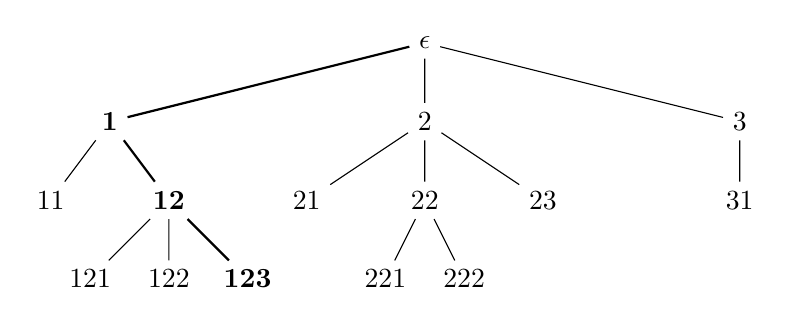
\begin{tikzpicture}[emph/.style={edge from parent/.style={draw,\maincolour,thick}},norm/.style={edge from parent/.style={draw,black,thin}}]
\node[\maincolour] {$\bm\epsilon$} [level 1/.style={sibling distance=4cm}, level 2/.style={sibling distance=1.5cm}, level 3/.style={sibling distance=1cm}, level distance=1cm]
	child[emph] {node[\maincolour] {\textbf{1}}
		child[norm] {node {11}}
		child[emph] {node[\maincolour] {\textbf{12}}
			child[norm] {node {121}}
			child[norm] {node {122}}
			child[emph] {node[\maincolour] {\textbf{123}}}
		}
	} 
	child {node {2}
		child {node {21}}
		child {node {22}
			child {node {221}}
			child {node {222}}
		}
		child {node {23}}
	}
	child {node {3}
		child {node {31}}
	};
\end{tikzpicture}
\end{center}

The address tape, then, contains symbols from the alphabet $\Sigma_{b}$. Each symbol on the address tape will tell $\mathcal{M}'$ which branch of the nondeterministic computation tree it must follow in its next computation step. Note that the contents of the address tape do not necessarily need to correspond to a vertex of the tree; if the address tape contains an invalid address, then $\mathcal{M}'$ simply aborts its attempted simulation of that branch.

Having defined the three tapes, we can describe how $\mathcal{M}'$ simulates the computation of $\mathcal{M}$:
\begin{enumerate}
\item Initialize the tapes in the following way: 
	\begin{enumerate}
	\item Copy the contents of the input tape to the simulation tape; that is, write the input word $w$ given to $\mathcal{M}$ to the simulation tape.
	\item Leave the address tape empty.
	\end{enumerate}
\item Use the simulation tape to perform the following steps:
	\begin{enumerate}
	\item For each computation step of $\mathcal{M}$, read the next symbol of the address tape to determine which branch of the nondeterministic computation tree to follow.
	\item If there are no more symbols remaining on the address tape, or if the address tape contains an invalid address, or if $\mathcal{M}$ enters a rejecting configuration, then abort the attempted simulation of this branch and go to step 3.
	\item If $\mathcal{M}$ enters an accepting configuration, then accept $w$.
	\end{enumerate}
\item Write to the address tape the sequence of symbols over $\Sigma_{b}$ that comes next in lexicographic order and go to step 2. \qedhere
\end{enumerate}
\end{proof}
\end{theorem}

Since every deterministic Turing machine is a nondeterministic Turing machine that doesn't use nondeterminism during its computation, we immediately obtain the other direction of the relationship between these models. Therefore, we can conclude that deterministic and nondeterministic Turing machines are equivalent.

\subsection{Multitape Turing Machines}

In the proof of Theorem~\ref{thm:NTMDTMequivalent}, we saw that we could simulate the computation of a nondeterministic Turing machine using a deterministic Turing machine with multiple tapes. It's natural to wonder whether including additional tapes gave us some kind of advantage in this simulation process---after all, giving our computational model two stacks instead of one stack led us to the idea of a Turing machine---but as it turns out, we can perform exactly the same computations using only a single tape.

First, let's define our \emph{multitape Turing machine} model. Again, we only need to modify the transition function: instead of mapping a pair of state and \emph{one} tape symbol to a tuple of state, \emph{one} tape symbol, and \emph{one} input head movement, we will transition on $k$ tape symbols and $k$ input head movements, where $k$ denotes the number of tapes used by the machine.

\begin{definition}[$k$-tape Turing machine]\label{def:multitapeTM}
A $k$-tape Turing machine is a tuple $(Q, \Sigma, \Gamma, \delta, q_{0}, q_{\text{accept}}, q_{\text{reject}})$, where everything is defined as in Definition~\ref{def:TM} except for the transition function, which is
\begin{equation*}
\delta: \left( Q \setminus \{q_{\text{accept}}, q_{\text{reject}}\} \right) \times \Gamma^{k} \to Q \times \Gamma^{k} \times \{L, R\}^{k}.
\end{equation*}
\end{definition}

The idea allowing us to establish one direction of the equivalence between multitape and single-tape Turing machines is that we can simulate having many tapes $T_{i}$ by storing all of the contents on a single tape $T$ and separating ``tape $i$" from the other ``tapes" using a special symbol. Since our single tape has only one input head, we will also simulate the position of each input head on ``tape $i$" using a special marker on the corresponding tape symbol to act as a virtual input head.

\begin{figure}
\centering
\begin{tikzpicture}[%
	tape1/.style={rectangle split, rectangle split horizontal, rectangle split parts=#1, rectangle split part align=base, draw, anchor=center, rectangle split part fill={white,white,white,white,white,\fourthcolour,white,white,white,white}},%
	tape2/.style={rectangle split, rectangle split horizontal, rectangle split parts=#1, rectangle split part align=base, draw, anchor=center, rectangle split part fill={white,white,white,white,\fourthcolour,white,white,white,white,white}},%
	tape3/.style={rectangle split, rectangle split horizontal, rectangle split parts=#1, rectangle split part align=base, draw, anchor=center, rectangle split part fill={white,\fourthcolour,white,white,white,white,white,white,white,white}}%
	]
\node[tape1=10] (tp1) {
\nodepart{one}$\cdots$
\nodepart{two}$\blankspace$
\nodepart{three}\texttt{a}
\nodepart{four}\texttt{b}
\nodepart{five}\texttt{b}
\nodepart{six}\color{\maincolour}\texttt{a}
\nodepart{seven}\texttt{a}
\nodepart{eight}\texttt{b}
\nodepart{nine}$\blankspace$
\nodepart{ten}$\cdots$
};
\node[tape2=10, below=0em of tp1] (tp2) {
\nodepart{one}$\cdots$
\nodepart{two}$\blankspace$
\nodepart{three}$\blankspace$
\nodepart{four}\texttt{0}
\nodepart{five}\color{\maincolour}\texttt{1}
\nodepart{six}\texttt{1}
\nodepart{seven}\texttt{0}
\nodepart{eight}$\blankspace$
\nodepart{nine}$\blankspace$
\nodepart{ten}$\cdots$
};
\node[tape3=10, below=0em of tp2] (tp3) {
\nodepart{one}$\cdots$
\nodepart{two}\color{\maincolour}\texttt{c}
\nodepart{three}\texttt{c}
\nodepart{four}\texttt{d}
\nodepart{five}\texttt{d}
\nodepart{six}\texttt{c}
\nodepart{seven}\texttt{c}
\nodepart{eight}\texttt{d}
\nodepart{nine}\texttt{d}
\nodepart{ten}$\cdots$
};
\end{tikzpicture}

\smallskip
$\Downarrow$
\medskip

\begin{tikzpicture}[tape/.style={fill=white, rectangle split, rectangle split horizontal, rectangle split parts=#1, rectangle split part align=base, draw, anchor=center}]
\node[tape=17] (tp) {
\nodepart{one}$\cdots$
\nodepart{two}$\blankspace$
\nodepart{three}\texttt{\#}
\nodepart{four}\texttt{a}
\nodepart{five}\texttt{b}
\nodepart{six}\texttt{b}
\nodepart{seven}$\bigdot{\texttt{a}}$
\nodepart{eight}\texttt{a}
\nodepart{nine}\texttt{b}
\nodepart{ten}\texttt{\#}
\nodepart{eleven}\texttt{0}
\nodepart{twelve}$\bigdot{\texttt{1}}$
\nodepart{thirteen}\texttt{1}
\nodepart{fourteen}\texttt{0}
\nodepart{fifteen}\texttt{\#}
\nodepart{sixteen}$\bigdot{\texttt{c}}$
\nodepart{seventeen}$\cdots$
};
\end{tikzpicture}
\caption{Simulating the computation of a $k$-tape Turing machine (top) with a single-tape Turing machine (bottom). The positions of the $k$ physical input heads are indicated by highlighted cells, while the corresponding $k$ virtual input heads are indicated by dots}
\label{fig:TMktapeto1tape}
\end{figure}

\begin{theorem}\label{thm:ktapeequivalent}
Given a $k$-tape Turing machine $\mathcal{M}$, we can construct a single-tape Turing machine $\mathcal{M}'$ such that $L(\mathcal{M}') = L(\mathcal{M})$.

\begin{proof}
Suppose the given Turing machine $\mathcal{M}$ has $k$ tapes, and the tape alphabet is denoted by $\Gamma$. Our single-tape Turing machine $\mathcal{M}'$ will simulate $\mathcal{M}$'s computation on an input word $w = w_{1} \dots w_{n}$ in the following way: 
\begin{enumerate}
\item Take the tape alphabet of $\mathcal{M}'$ to be $\Gamma' = \Gamma \cup \bigdot{\Gamma} \cup \{\texttt{\#}\}$, where $\bigdot{\Gamma}$ consists of all alphabet symbols of $\Gamma$ augmented with a dot and \texttt{\#} is a special boundary marker.
\item Write the boundary marker \texttt{\#} and the symbols of $w$ to the tape of $\mathcal{M}'$, including the dotted symbol $\bigdot{w_{1}}$. Then, write $k+1$ copies of \texttt{\#} each separated by a dotted blank space.
\begin{center}
\begin{tikzpicture}[tape/.style={fill=white, rectangle split, rectangle split horizontal, rectangle split parts=#1, rectangle split part align=base, draw, anchor=center}]
\node[tape=12] (tp) {
\nodepart{one}$\cdots$
\nodepart{two}$\blankspace$
\nodepart{three}\texttt{\#}
\nodepart{four}$\bigdot{w_{1}}$
\nodepart{five}$\dots$
\nodepart{six}$w_{n}$
\nodepart{seven}\texttt{\#}
\nodepart{eight}$\bigdot{\blankspace}$
\nodepart{nine}\texttt{\#}
\nodepart{ten}$\bigdot{\blankspace}$
\nodepart{eleven}\texttt{\#}
\nodepart{twelve}$\cdots$
};
\end{tikzpicture}
\end{center}
\item For each step of the computation, $\mathcal{M}'$ scans its entire tape from the first occurrence of \texttt{\#} to the $(k+1)$st occurrence of \texttt{\#} to read the symbols on all $k$ tapes of $\mathcal{M}$. Then, $\mathcal{M}'$ makes a second pass along its tape to update any symbols that were changed by the transition function of $\mathcal{M}$. This update includes changing occurrences of dotted symbols in accordance with the changed positions of each virtual input head.

If any of the virtual input heads of $\mathcal{M}'$ move onto an occurrence of \texttt{\#}, then $\mathcal{M}$ must have moved the corresponding input head of that tape onto a blank space. In this case, $\mathcal{M}'$ writes a blank space to this cell of its tape and shifts the symbols of all subsequent cells rightward by one position. \qedhere
\end{enumerate}
\end{proof}
\end{theorem}

The process of condensing the contents of all $k$ tapes onto a single tape is illustrated in Figure~\ref{fig:TMktapeto1tape}. Naturally, a $k$-tape Turing machine can simulate the computation of a single-tape Turing machine by using only one of its $k$ tapes. This again gives us the other direction of the relationship between the models, and again establishes the equivalence of the models.

\subsection{One-Way Infinite Tape Turing Machines}

In our definition of a Turing machine, we assumed that the tape used by the machine is \emph{two-way infinite}; that is, there is an infinite number of cells to the left and to the right of the input head, and the input head can therefore move to an infinite number of positions of the tape in either direction.

We didn't have to define our storage in this way, though. We could have alternatively defined the tape to act more like the stack of a pushdown automaton: just like the stack has a fixed bottom boundary forcing us to push symbols only above that boundary, the tape could have a fixed left boundary forcing us to write symbols only to the right of that boundary. We call such a tape \emph{one-way infinite}, since at any position along the tape, the input head has a finite number of cells to its left and an infinite number of cells to its right.

Because of the way the computation of the Turing machine begins, the initial position of the input head of a Turing machine with a one-way infinite tape will be on the first symbol of the input word, and the left boundary of the tape will be to the input head's immediate left. In this cell, the input head cannot make a leftward move; if the transition function tells the input head to move left, then the input head will simply remain in the same cell by making a rightward move immediately followed by a leftward move.

\begin{remark}
Some authors alternatively assert that, if the input head of a one-way infinite tape Turing machine moves beyond the left boundary of the tape, then the machine ``crashes" and the computation cannot continue.
\end{remark}

If we want to simulate the computation of a one-way infinite tape Turing machine using a two-way infinite tape Turing machine, then the required conversion seems straightforward: we just need to write a special symbol to one cell of the two-way infinite tape to act as the left boundary, and modify the transition function to handle the case where the input head moves onto this left boundary marker.

\begin{figure}
\centering
\begin{tikzpicture}[tape/.style={fill=white, rectangle split, rectangle split horizontal, rectangle split parts=#1, rectangle split part align=base, draw, anchor=center}]
\node[tape=6] (tp) {
\nodepart{one}\texttt{a}
\nodepart{two}\texttt{b}
\nodepart{three}\texttt{b}
\nodepart{four}\texttt{a}
\nodepart{five}$\blankspace$
\nodepart{six}$\cdots$
};
\end{tikzpicture}

\smallskip
$\Downarrow$
\medskip

\begin{tikzpicture}[tape/.style={fill=white, rectangle split, rectangle split horizontal, rectangle split parts=#1, rectangle split part align=base, draw, anchor=center}]
\node[tape=10] (tp) {
\nodepart{one}$\cdots$
\nodepart{two}$\blankspace$
\nodepart{three}$\blankspace$
\nodepart{four}$\vdash$
\nodepart{five}\texttt{a}
\nodepart{six}\texttt{b}
\nodepart{seven}\texttt{b}
\nodepart{eight}\texttt{a}
\nodepart{nine}$\blankspace$
\nodepart{ten}$\cdots$
};
\end{tikzpicture}
\caption{Simulating the computation of a one-way infinite tape Turing machine (top) with a two-way infinite tape Turing machine (bottom)}
\label{fig:TMonewaytotwoway}
\end{figure}

\begin{theorem}\label{thm:onewayequivalent}
Given a one-way infinite tape Turing machine $\mathcal{M}$, we can construct a two-way infinite tape Turing machine $\mathcal{M}'$ such that $L(\mathcal{M}') = L(\mathcal{M})$.

\begin{proof}
Suppose the given one-way infinite tape Turing machine $\mathcal{M}$ receives as input a word $w = w_{1} \dots w_{n}$ and has a tape alphabet $\Gamma$. Our two-way infinite tape Turing machine $\mathcal{M}'$ will simulate $\mathcal{M}$'s computation on $w$ in the following way:
\begin{enumerate}
\item Take the tape alphabet of $\mathcal{M}'$ to be $\Gamma' = \Gamma \cup \{\vdash\}$, where $\vdash$ is a special left boundary marker.
\item Write the symbols of $w$ to the tape of $\mathcal{M}'$, and write the left boundary marker $\vdash$ in the cell to the immediate left of the cell containing $w_{1}$.
\item Take the transition function of $\mathcal{M}'$ to be $\delta' = \delta$ and, for each state $q \in Q$, add a new transition $\delta'(q, \vdash) = (q, \vdash, R)$ to the transition function of $\mathcal{M}'$.
\item Create new states $q'_{\text{accept}}$ and $q'_{\text{a}}$, and add new transitions to the transition function of $\mathcal{M}'$ as follows:
	\begin{itemize}
	\item $\delta'(q_{\text{accept}}, \vdash) = (q'_{\text{accept}}, \vdash, R)$;
	\item $\delta'(q_{\text{accept}}, c) = (q'_{\text{a}}, c, R)$ for all $c \in \Gamma' \setminus \{\vdash\}$; and
	\item $\delta'(q'_{\text{a}}, d) = (q'_{\text{accept}}, d, L)$ for all $d \in \Gamma' \setminus \{\vdash\}$.
	\end{itemize}
Also, create new states $q'_{\text{reject}}$ and $q'_{\text{r}}$, and add similar transitions on these states. Take the accepting and rejecting states of $\mathcal{M}'$ to be $q'_{\text{accept}}$ and $q'_{\text{reject}}$, respectively. \qedhere
\end{enumerate}
\end{proof}
\end{theorem}

The construction described in Theorem~\ref{thm:onewayequivalent} is illustrated in Figure~\ref{fig:TMonewaytotwoway}.

\begin{figure}
\centering
\begin{tikzpicture}[tape/.style={fill=white, rectangle split, rectangle split horizontal, rectangle split parts=#1, rectangle split part align=base, draw, anchor=center}]
\node[tape=10] (tp) {
\nodepart{one}$\cdots$
\nodepart{two}$\blankspace$
\nodepart{three}$\blankspace$
\nodepart{four}\texttt{a}
\nodepart{five}\texttt{b}
\nodepart{six}\texttt{b}
\nodepart{seven}\texttt{a}
\nodepart{eight}\texttt{a}
\nodepart{nine}\texttt{b}
\nodepart{ten}$\cdots$
};
\end{tikzpicture}

\smallskip
$\Downarrow$
\medskip

\begin{tikzpicture}[tape/.style={fill=white, rectangle split, rectangle split horizontal, rectangle split parts=#1, rectangle split part align=base, draw, anchor=center}]
\node[tape=8] (tp1) {
\nodepart{one}\texttt{a}
\nodepart{two}\texttt{b}
\nodepart{three}\texttt{b}
\nodepart{four}\texttt{a}
\nodepart{five}\texttt{a}
\nodepart{six}\texttt{b}
\nodepart{seven}$\blankspace$
\nodepart{eight}$\cdots$
};
\node[tape=8, below=0em of tp1] (tp2) {
\nodepart{one}$\blankspace$
\nodepart{two}$\blankspace$
\nodepart{three}$\blankspace$
\nodepart{four}$\blankspace$
\nodepart{five}$\blankspace$
\nodepart{six}$\blankspace$
\nodepart{seven}$\blankspace$
\nodepart{eight}$\cdots$
};
\path[<->, >=latex, color=\maincolour] ($(tp1.west)+(-0.2,0)$) edge[thick, bend right=90, min distance=1.25em] ($(tp2.west)+(-0.2,0)$);
\end{tikzpicture}
\caption{Simulating the computation of a two-way infinite tape Turing machine (top) with a one-way infinite tape Turing machine (bottom)}
\label{fig:TMtwowaytooneway}
\end{figure}

To obtain the other direction of the equivalence---that is, to simulate the computation of a two-way infinite tape Turing machine with a one-way infinite tape Turing machine---we can use our previous result establishing the equivalence of single-tape and multitape Turing machines.

While we won't go through the full proof here, the idea is to split the two-way infinite tape into a pair of one-way infinite tapes, where the ``split point" occurs between the first symbol of the input word and the infinite blank spaces to the left of the input word. This action produces two one-way infinite tapes: one containing the input word, and one containing only blank spaces. Then, we modify the transition function of the one-way infinite tape Turing machine to operate on either the first or second tape, switching between the tapes each time the input head of the two-way infinite tape Turing machine crosses the ``split point" on its tape.

Splitting the two-way infinite tape into a pair of one-way infinite tapes gives us the setup depicted in Figure~\ref{fig:TMtwowaytooneway}, where the two-way infinite tape is, in effect, folded in half. Ultimately, this construction completes the proof and establishes the equivalence between one-way and two-way infinite tape Turing machines.

%\subsection{Turing Machines with No-Ops}
\futuresection{Closure Properties}\label{sec:closurepropertiesdecidable}

\begin{construction}
As with the previous chapters, I eventually plan to write a section summarizing the closure properties of various operations applied to the classes of decidable and semidecidable languages. Since Turing machines are so powerful, it's not surprising that nearly all operations are closed for both decidable and semidecidable languages, but it's worth explaining that semidecidable languages happen not to be closed under complement.
\end{construction}
\futuresection{Encodings of Turing Machines}\label{sec:encodingturingmachines}

\begin{construction}
In advance of the section on universal Turing machines, I plan to write a short exposition on arithmetization and ways in which we might encode a description of a Turing machine as a string of symbols $\langle \mathcal{M} \rangle$.
\end{construction}
\section{Universal Turing Machines}\label{sec:universalturingmachines}

\firstwords{Up to now}, we have had to construct different specific Turing machines for each language we wished to recognize. In fact, we have had to construct specific machines for \emph{every} language we wished to recognize in this course, whether that machine be a finite automaton, or a pushdown automaton, or indeed, a Turing machine.

However, we know that Turing machines are capable of performing quite complicated computations, and we know also that we can construct Turing machines that can simulate the computations of other variant Turing machines. What if we took this idea and generalized it as much as possible? That is, what if we constructed some Turing machine that could simulate the computation of \emph{any} other Turing machine?

Alan Turing considered this exact idea in the paper that introduced the model of computation that would eventually be named after him. Turing described the process of constructing a machine $\mathcal{U}$ that is capable of simulating the computation of any other machine $\mathcal{M}$, so long as we give an appropriate encoding of $\mathcal{M}$ as part of the input to $\mathcal{U}$: \par
\epigraph{It is possible to invent a single machine which can be used \par
to compute any computable sequence. If this machine U \par
is supplied with a tape on the beginning of which is written \par
the S.D.\ [standard description] of some computing machine M, \par
then U will compute the same sequence as M.}{Alan Turing}{On Computable Numbers, with an Application to the Entscheidungsproblem}{}
\vspace{1em}
\noindent
Here, like Turing did before us, we will show how to construct such a machine $\mathcal{U}$, which is nowadays called a \emph{universal Turing machine}.

\begin{remark}
It's important to note that, in this context, ``universal" does not mean that the Turing machine $\mathcal{U}$ can compute \emph{everything}. It only means that $\mathcal{U}$ can compute whatever other Turing machines can compute.
\end{remark}

The main benefit of having such a machine is that we will no longer have to construct specific Turing machines for each language we consider; now, we can just give a high-level description of the Turing machine's computation, and we can feasibly ``program" the universal Turing machine to perform its computation in a similar way. These high-level descriptions will be quite similar to what we saw in the proofs of Theorems~\ref{thm:NTMDTMequivalent}, \ref{thm:ktapeequivalent}, and \ref{thm:onewayequivalent}, where we simply listed the steps of the machine's computation instead of explicitly writing out each component of the machine.

Suppose that the input we give to our universal Turing machine $\mathcal{U}$ is of the form $\langle \mathcal{M}, w \rangle$, where $\mathcal{M}$ is an encoding of the Turing machine we wish to simulate and $w$ is the input word given to $\mathcal{M}$. Given an input of this form, our machine $\mathcal{U}$ must satisfy three criteria:
\begin{colouredbox}
\begin{enumerate}
\item $\mathcal{U}$ halts its computation on input $\langle \mathcal{M}, w \rangle$ if and only if $\mathcal{M}$ halts its computation on input $w$;
\item $\mathcal{U}$ enters its accepting state if and only if $\mathcal{M}$ enters its accepting state; and
\item $\mathcal{U}$ enters its rejecting state if and only if $\mathcal{M}$ enters its rejecting state.
\end{enumerate}
\end{colouredbox}

We now go through with the construction of this machine $\mathcal{U}$.

\begin{theorem}
There exists a universal Turing machine $\mathcal{U}$ that, given an input $\langle \mathcal{M}, w \rangle$, is capable of simulating the computation of a Turing machine $\mathcal{M}$ on an input word $w$.

\begin{proof}
We will construct $\mathcal{U}$ in the form of a multitape Turing machine, just as we did in our procedure to determinise a nondeterministic Turing machine.

For this construction, we need only three tapes:
\begin{itemize}
\item The first tape will initially contain the input $\langle \mathcal{M}, w \rangle$, and after the computation of $\mathcal{U}$ begins, it will simulate the contents of the tape of $\mathcal{M}$.
\item The second tape will contain the encoding of the machine $\mathcal{M}$.
\item The third tape will keep track of which state we are currently in during the computation of $\mathcal{M}$ by maintaining the current state as a binary number.
\end{itemize}

At the beginning of its computation, $\mathcal{U}$ will contain only the input $\langle \mathcal{M}, w \rangle$ on its first tape, and its other two tapes will be blank.

\begin{center}
\begin{tikzpicture}[tape/.style={fill=white, rectangle split, rectangle split horizontal, rectangle split parts=#1, rectangle split part align=base, draw, anchor=center}]
\node[tape=13] (tp) {
\nodepart{one}$\cdots$
\nodepart{two}$\blankspace$
\nodepart{three}\hspace*{0.75pt}$\langle$\hspace*{0.75pt}
\nodepart{four}\raisebox{1pt}{\makebox[0.52em][c]{.\hfil.\hfil.}}
\nodepart{five}\hspace*{-2pt}\footnotesize$\mathcal{M}$\hspace*{-2.1pt}
\nodepart{six}\raisebox{1pt}{\makebox[0.52em][c]{.\hfil.\hfil.}}
\nodepart{seven}\hspace*{1.25pt},\hspace*{1.25pt}
\nodepart{eight}\raisebox{1pt}{\makebox[0.52em][c]{.\hfil.\hfil.}}
\nodepart{nine}\hspace*{-1.1pt}$w$\hspace*{-1.1pt}
\nodepart{ten}\raisebox{1pt}{\makebox[0.52em][c]{.\hfil.\hfil.}}
\nodepart{eleven}\hspace*{0.75pt}$\rangle$\hspace*{0.75pt}
\nodepart{twelve}$\blankspace$
\nodepart{thirteen}$\cdots$
};
\end{tikzpicture}
\begin{tikzpicture}[tape/.style={fill=white, rectangle split, rectangle split horizontal, rectangle split parts=#1, rectangle split part align=base, draw, anchor=center}]
\node[tape=13] (tp) {
\nodepart{one}$\cdots$
\nodepart{two}$\blankspace$
\nodepart{three}$\blankspace$
\nodepart{four}\raisebox{1pt}{\makebox[0.52em][c]{.\hfil.\hfil.}}
\nodepart{five}$\blankspace$
\nodepart{six}\raisebox{1pt}{\makebox[0.52em][c]{.\hfil.\hfil.}}
\nodepart{seven}$\blankspace$
\nodepart{eight}\raisebox{1pt}{\makebox[0.52em][c]{.\hfil.\hfil.}}
\nodepart{nine}$\blankspace$
\nodepart{ten}\raisebox{1pt}{\makebox[0.52em][c]{.\hfil.\hfil.}}
\nodepart{eleven}$\blankspace$
\nodepart{twelve}$\blankspace$
\nodepart{thirteen}$\cdots$
};
\end{tikzpicture}
\begin{tikzpicture}[tape/.style={fill=white, rectangle split, rectangle split horizontal, rectangle split parts=#1, rectangle split part align=base, draw, anchor=center}]
\node[tape=13] (tp) {
\nodepart{one}$\cdots$
\nodepart{two}$\blankspace$
\nodepart{three}$\blankspace$
\nodepart{four}\raisebox{1pt}{\makebox[0.52em][c]{.\hfil.\hfil.}}
\nodepart{five}$\blankspace$
\nodepart{six}\raisebox{1pt}{\makebox[0.52em][c]{.\hfil.\hfil.}}
\nodepart{seven}$\blankspace$
\nodepart{eight}\raisebox{1pt}{\makebox[0.52em][c]{.\hfil.\hfil.}}
\nodepart{nine}$\blankspace$
\nodepart{ten}\raisebox{1pt}{\makebox[0.52em][c]{.\hfil.\hfil.}}
\nodepart{eleven}$\blankspace$
\nodepart{twelve}$\blankspace$
\nodepart{thirteen}$\cdots$
};
\end{tikzpicture}
\end{center}

Now, we can describe how $\mathcal{U}$ simulates the computation of $\mathcal{M}$ on $w$:
\begin{enumerate}
\item Initialize the tapes in the following way:
	\begin{enumerate}
	\item Transfer the encoding of $\mathcal{M}$ from the first tape to the second tape by writing $\langle \mathcal{M} \rangle$ to the second tape and erasing it from the first tape.
	\item Read the encoding of $\mathcal{M}$ on the second tape to determine the number of states in $\mathcal{M}$. If $\mathcal{M}$ contains $k$ states, then write $\lceil\log_{2}(k)\rceil$ copies of \texttt{0} to the third tape.
	
	\textit{(Remember, the current state is being maintained as a binary number, so we need a logarithmic amount of bits to represent a given state's number $k$.)}
	\end{enumerate}
	
After initialization, the tape will look like the following:
\begin{center}
\begin{tikzpicture}[tape/.style={fill=white, rectangle split, rectangle split horizontal, rectangle split parts=#1, rectangle split part align=base, draw, anchor=center}]
\node[tape=13] (tp) {
\nodepart{one}$\cdots$
\nodepart{two}$\blankspace$
\nodepart{three}$\blankspace$
\nodepart{four}\raisebox{1pt}{\makebox[0.52em][c]{.\hfil.\hfil.}}
\nodepart{five}$\blankspace$
\nodepart{six}\raisebox{1pt}{\makebox[0.52em][c]{.\hfil.\hfil.}}
\nodepart{seven}\hspace*{0.75pt}$\langle$\hspace*{0.75pt}
\nodepart{eight}\raisebox{1pt}{\makebox[0.52em][c]{.\hfil.\hfil.}}
\nodepart{nine}\hspace*{-1.1pt}$w$\hspace*{-1.1pt}
\nodepart{ten}\raisebox{1pt}{\makebox[0.52em][c]{.\hfil.\hfil.}}
\nodepart{eleven}\hspace*{0.75pt}$\rangle$\hspace*{0.75pt}
\nodepart{twelve}$\blankspace$
\nodepart{thirteen}$\cdots$
};
\end{tikzpicture}
\begin{tikzpicture}[tape/.style={fill=white, rectangle split, rectangle split horizontal, rectangle split parts=#1, rectangle split part align=base, draw, anchor=center}]
\node[tape=13] (tp) {
\nodepart{one}$\cdots$
\nodepart{two}$\blankspace$
\nodepart{three}\hspace*{0.75pt}$\langle$\hspace*{0.75pt}
\nodepart{four}\raisebox{1pt}{\makebox[0.52em][c]{.\hfil.\hfil.}}
\nodepart{five}\hspace*{-2pt}\footnotesize$\mathcal{M}$\hspace*{-2.1pt}
\nodepart{six}\raisebox{1pt}{\makebox[0.52em][c]{.\hfil.\hfil.}}
\nodepart{seven}\hspace*{0.75pt}$\rangle$\hspace*{0.75pt}
\nodepart{eight}\raisebox{1pt}{\makebox[0.52em][c]{.\hfil.\hfil.}}
\nodepart{nine}$\blankspace$
\nodepart{ten}\raisebox{1pt}{\makebox[0.52em][c]{.\hfil.\hfil.}}
\nodepart{eleven}$\blankspace$
\nodepart{twelve}$\blankspace$
\nodepart{thirteen}$\cdots$
};
\end{tikzpicture}
\begin{tikzpicture}[tape/.style={fill=white, rectangle split, rectangle split horizontal, rectangle split parts=#1, rectangle split part align=base, draw, anchor=center}]
\node[tape=13] (tp) {
\nodepart{one}$\cdots$
\nodepart{two}$\blankspace$
\nodepart{three}\texttt{0}
\nodepart{four}\raisebox{1pt}{\makebox[0.52em][c]{.\hfil.\hfil.}}
\nodepart{five}\texttt{0}
\nodepart{six}\raisebox{1pt}{\makebox[0.52em][c]{.\hfil.\hfil.}}
\nodepart{seven}\texttt{0}
\nodepart{eight}\raisebox{1pt}{\makebox[0.52em][c]{.\hfil.\hfil.}}
\nodepart{nine}$\blankspace$
\nodepart{ten}\raisebox{1pt}{\makebox[0.52em][c]{.\hfil.\hfil.}}
\nodepart{eleven}$\blankspace$
\nodepart{twelve}$\blankspace$
\nodepart{thirteen}$\cdots$
};
\end{tikzpicture}
\end{center}
\item Move the input head of the first tape to the first symbol of $w$. Move the input head of the second tape to the first symbol of $\langle \mathcal{M} \rangle$. Move the input head of the third tape to the first symbol of the sequence of \texttt{0}s.
\item Repeat the following steps until $\mathcal{M}$ halts:
	\begin{enumerate}
	\item For each computation step of $\mathcal{M}$, scan the second tape to find a transition that matches the current input symbol and state written on the first and third tapes, respectively.
	\item Modify the contents of the first and third tapes to reflect the transition that was just taken.
	\item If no transition exists for the current state/symbol pair, then halt and go to step 4.
	\end{enumerate}
\item Transition to $q_{\text{accept}}$ if $\mathcal{M}$ transitioned to its accepting state. Transition to $q_{\text{reject}}$ if $\mathcal{M}$ transitioned to its rejecting state. \qedhere
\end{enumerate}
\end{proof}
\end{theorem}

Let's now verify that this construction does, in fact, satisfy the three criteria we laid out earlier. First, we require that $\mathcal{U}$ halts its computation on input $\langle \mathcal{M}, w \rangle$ if and only if $\mathcal{M}$ halts its computation on input $w$. Since $\mathcal{U}$ uses the description of $\mathcal{M}$ to see what it would do after reading each symbol of $w$, $\mathcal{U}$ behaves in a manner identical to $\mathcal{M}$, and so $\mathcal{U}$ halts on its input if and only if $\mathcal{M}$ also halts on its input. Second, we require that $\mathcal{U}$ accepts if and only if $\mathcal{M}$ accepts, and we see immediately that this happens by Step 4 of the simulation procedure. In fact, $\mathcal{U}$ can't reach its accepting state unless $\mathcal{M}$ has done the same. Third, we require the same behaviour for rejecting inputs, and the argument in this case is nearly identical to the one we had for accepting inputs. Therefore, the universal Turing machine $\mathcal{U}$ satisfies all of our criteria and performs a correct simulation of any other Turing machine we provide as input!
\section{The Church--Turing Thesis}\label{sec:churchturingthesis}

\firstwords{Long ago}, before digital computers as we know them existed and even before the phrase ``computer science" entered the lexicon of humanity, mathematicians and logicians wanted to know whether it was possible to use mechanical procedures to solve mathematical problems. The desire for such procedures dates back to the 17th century and the time of Gottfried Wilhelm Leibniz, who dreamt of constructing a machine he called a \emph{calculus ratiocinator} to automate the task of performing general mathematical calculations. (Although Leibniz is well-known for his work on \emph{the} calculus of infinitesimals that one often learns in school, the word ``calculus" in this sense refers more generally to a system for performing calculations.)

Leibniz's ratiocinator was to use a formal language he called \emph{characteristica universalis}---Latin for ``universal character"---which he intended to be a general framework for expressing mathematical concepts in symbols. Indeed, the characteristica universalis might be considered the first programming language! Although Leibniz never succeeded in constructing his ratiocinator, his dream formed the precursor for much of the work done in the formalization of mathematics throughout the 19th and 20th centuries.

At the turn between these two centuries, David Hilbert delivered a presentation to the International Congress of Mathematicians~\citeyearpar{Hilbert1900MathematischeProbleme, Hilbert1901MathematischeProbleme} wherein he outlined 10 (and later, an additional 13) unsolved problems that would come to guide the new century's study of mathematics. Of Hilbert's 23 problems, three remain unsolved to this day, while two are considered too vague to ever have a proper solution. But one problem in particular is relevant to our current topic: the \emph{second problem}, which asks to prove that the axioms of arithmetic over the real numbers are consistent; that is, incapable of producing logical contradictions.

Much like Leibniz dreamt of a machine to solve any mathematical problem, Hilbert dreamt of a purely logical formal system where, starting from a given set of axioms, one would be able to prove any mathematical statement. Indeed, this dream motivated his second problem: if the axioms of arithmetic are consistent, then we can use pure logical rules to solve any mathematical problem we come across.\par
\epigraph{We hear within us the perpetual call:\par
There is the problem. Seek its solution.\par
You can find it by pure reason, for\par
in mathematics there is no ignorabimus.}{David Hilbert}{Mathematical Problems}{}
\vspace{1em}
\noindent
In the following decades, Hilbert devoted considerable time to trying to establish a positive answer for his second problem. Unfortunately for him, Kurt G\"{o}del would show via his \emph{incompleteness theorems}~\citeyearpar{Godel1931UberFormalUnentscheidbare} not just that a proof of consistency for even a simpler system like the Peano arithmetic over the natural numbers is impossible to attain within the system itself, but also that such arithmetic systems \emph{must} contain statements that can be neither proved nor disproved. In resolving the second problem in the negative, G\"{o}del dealt a crushing blow to Hilbert's dream: in mathematics, it turns out there \emph{is} some ignorabimus. Despite this substantial setback, Hilbert and others persisted in looking forward, and researchers continued pursuing modified and constrained forms of Hilbert's dream---even if we can't formalize all of mathematics, we can at least formalize some of mathematics.

A few years before G\"{o}del announced his groundbreaking results, Hilbert---together with his doctoral student Wilhelm Ackermann---posed a more concrete question in their book, \textit{Grundz\"{u}ge der theoretischen Logik}~\citeyearpar{HilbertAckermann1928Grundzuge}. Their question, closer in spirit to Leibniz's dream, asked for\par
\epigraph{\textup{[\,\dots]} a method which permits us to decide for any given formula\par
in which domains of individuals it is universally valid (or satisfiable)\par
and in which it is not.}{David Hilbert and Wilhelm Ackermann}{Grundz\"{u}ge der theoretischen Logik (translated edition, 1950)}{}
\vspace{1em}
\noindent
In other words, Hilbert and Ackermann wanted to know whether there exists a general procedure that takes a predicate logic formula and gives a ``yes" or ``no" answer as to whether that formula is true, no matter which predicates are used or which values are assigned to variables within the formula. Their question would come to be known as the \emph{Entscheidungsproblem}, which is German for ``decision problem". Although G\"{o}del's work had brought down Hilbert's second problem, researchers at the time noted that, strictly speaking, the Entscheidungsproblem had not suffered the same fate. There remained, at least for the time being, a glimmer of hope.

The issue, however, was that there was not yet a universally agreed-upon definition of a ``procedure" that could decide such a thing as the Entscheidungsproblem. The most appropriate definition was eventually taken to be that of an \emph{effective method}. If we're given a class of problems, then a method for that class of problems is called effective if
\begin{colouredbox}
\begin{enumerate}
\item the method consists of a finite number of exact instructions; and
\item the method always terminates and produces a correct answer when it is applied to a problem from its class.
\end{enumerate}
\end{colouredbox}
In principle, an effective method is one that a human can perform on paper in a purely mechanical manner; it requires no creative thought or insight to arrive at an answer. It is computation in its purest form. If we view the class of problems in a way that allows us to map individual inputs to ``yes" and ``no" outputs, then we obtain a function for that class, and we say that such a function is \emph{effectively calculable}.

\begin{remark}
Compare our characterization of an effectively calculable function to the properties of a computable function given by~\citet{Enderton1977ElementsRecursionTheory} in Section~\ref{subsec:computingfunctions}. Criteria 1 and 2 match almost exactly!
\end{remark}

But what specific properties does an effectively calculable function possess? In a lecture given in 1934, whose notes were published decades later by Davis~\citeyearpar{Godel1934UndecidablePropositions}, G\"{o}del proposed that the notion of effective calculability could be captured by the so-called \emph{general recursive} functions. In doing so, he provided at least an initial characterization of what it means for a function to be effectively calculable. However, this was to be only the first step in a series of consequential results pertaining to the Entscheidungsproblem.

The first major breakthrough for the Entscheidungsproblem came in a series of papers by Alonzo Church, who framed the idea of effective calculability in terms of his \emph{lambda calculus}. The lambda calculus is a logical system that allows us to express computations in terms of functions and their applications. As it turns out, the class of effectively calculable functions corresponds to the class of functions that are expressible in the lambda calculus; this was formally established by both \citet{Church1936UnsolvableProblemNumberTheory} and \citet{Kleene1936GeneralRecursiveFunctions, Kleene1936LambdaDefinability}. Church ultimately proved that there does not exist any procedure to decide whether a given formula has an equivalent particular normal form in the lambda calculus~\citeyearpar{Church1936NoteEntscheidungsproblem, Church1936UnsolvableProblemNumberTheory}. From this observation, Church struck at Hilbert's dream once again and concluded the following:\par
\epigraph{The general case of the Entscheidungsproblem\par
of the engere Funktionenkalk\"{u}l is unsolvable.}{Alonzo Church}{A Note on the Entscheidungsproblem}{}
\vspace{1em}

The second breakthrough came with a presentation by Alan Turing to the London Mathematical Society~\citeyearpar{Turing1936OnComputableNumbers}. Like Church, Turing showed:\par
\epigraph{\textup{[\,\dots]} the Hilbertian Entscheidungsproblem can have no solution.}{Alan Turing}{On Computable Numbers, with an Application to the Entscheidungsproblem}{}
\vspace{1em}
\noindent
However, Turing relied on a different formalization: a machine model, which later came to be known as our familiar \emph{Turing machine}. The crux of Turing's argument was that the Entscheidungsproblem could be reformulated, or \emph{reduced}, to a problem pertaining to a property of his machine, and one could then show that this problem is also unsolvable. Turing was aware of Church's work---indeed, he raced to deliver his presentation shortly after learning about Church's work in that same year---and Turing added as an appendix to his published paper a proof sketch showing that his machine formalization was equivalent to Church's lambda calculus, and therefore to the class of effectively calculable functions. Turing would go on to earn his doctorate under the supervision of Church just a couple of years later.

Despite this flurry of results and the fall of the Entscheidungsproblem, there remained a question: G\"{o}del had the general recursive functions, Church had the lambda calculus, and Turing had his machines, but which of these formulations is best to use when we refer to effective calculability? This question was not truly settled until the following decade, when Stephen Kleene made the claim that \emph{any} of these formulations is suitable. Kleene~\citeyearpar{Kleene1943RecursivePredicates} began by introducing what he calls \emph{Church's thesis}:\par
\epigraph{Every effectively calculable function \par
(effectively decidable predicate) \par
is general recursive.}{Stephen Kleene}{Recursive Predicates and Quantifiers}{}
\vspace{1em}
\noindent
Church's thesis connects the class of general recursive functions to the lambda calculus by stating, in our terminology, that any problem for which there exists a procedure that returns an answer on each input belonging to the problem's language is semidecidable.

Kleene later introduced in his book \textit{Introduction to Metamathematics}~\citeyearpar{Kleene1952IntroductionToMetamathematics} a companion statement, which he calls \emph{Turing's thesis}:\par
\epigraph{\textup{[\,\dots]} that every function which would naturally be regarded \par
as computable under [Turing's] definition, i.e. by one of \par
his machines, is equivalent to Church's thesis \textup{[\,\dots]}}{Stephen Kleene}{Introduction to Metamathematics}{}
\vspace{1em}
\noindent
Turing's thesis is Kleene's encapsulation of what Turing himself expressed in the appendix of his paper: that his machine formalization is equivalent to the lambda calculus formalization given by Church. Consequently, anything that a Turing machine can do is effectively calculable, and therefore it is semidecidable.

Taken together, these two statements give us the \emph{Church--Turing thesis}: the unifier between effective methods and Turing machines. In modern language, we can express the thesis as follows.
\begin{customtitlebox}[Church--Turing thesis]
Any function that can be computed by an algorithm can also be computed on a Turing machine.
\end{customtitlebox}
\noindent
Note that we refer to this result as a ``thesis" and not as a ``theorem", since it is more definitional rather than a statement that we can formally prove.

\subsubsection*{Turing-Completeness}

In recent times, the Church--Turing thesis has allowed researchers to prove that all sorts of formal models are capable of behaving like a machine running an algorithm. If some model of computation or some system of rules can be used in a way that allows it to simulate the computation of any Turing machine, then we say that model or system is \emph{Turing-complete}.

We've already seen one example of something that is Turing-complete---the universal Turing machine. But since that is itself a kind of Turing machine, we shouldn't be too surprised. Instead, there are many more (and much weirder) examples of Turing-complete things in our daily lives:
\begin{colouredbox}
\begin{itemize}
\item Most general-purpose programming languages, and some specialized languages (like \LaTeX, the typesetting system used to create this book!)
\item Microsoft Excel and Microsoft PowerPoint
\item Conway's Game of Life and other cellular automata
\item Enzyme-based DNA computers
\item The cells of the human heart
\item The Dwarf Fortress, Minecraft, and Minesweeper video games
\item The Magic: The Gathering card game
\item The x86 assembler instruction \texttt{mov}, by itself
\end{itemize}
\end{colouredbox}
You might now reasonably wonder whether the computers we use every day are Turing-complete. Well, the answer---strictly speaking---is no! This comes down to one simple reason: nobody has figured out how to equip a real-world computer with an infinite amount of memory. Thus, when we speak about something being Turing-complete, we often set aside the limitation of finite memory and focus on the computational power of the thing itself.
\section{The Chomsky Hierarchy}\label{sec:chomskyhierarchy}

\begin{construction}
I plan to expand this short section about the Chomsky hierarchy to tie together all that we have learned about language classes and models of computation.
\end{construction}

The Chomsky hierarchy was initially proposed by Noam Chomsky~\citeyearpar{Chomsky1956ThreeModels, Chomsky1959FormalPropertiesGrammars} and further refined in Chomsky's joint work with the mathematician Marcel-Paul Sch\"{u}tzenberger~\citeyearpar{ChomskySchutzenberger1963ContextFree}. There are two major differences between the hierarchy we developed and Chomsky's hierarchy: in our hierarchy, we included the class of finite languages as a subset of the regular languages, while Chomsky's hierarchy includes the class of \emph{context-sensitive languages} that we briefly discussed, but otherwise left aside.

\begin{table}
\centering
\caption{The Chomsky hierarchy}
\label{tab:chomskyhierarchy}
\begin{tabular}{l l l}
\toprule
\textbf{Language class}	& \textbf{Model of computation}		& \textbf{Grammar} \\
\midrule
Recursively enumerable	& Turing machines				& Type 0 \\
Context-sensitive		& Linear-bounded automata		& Type 1 \\
Context-free			& Pushdown automata			& Type 2 \\
Regular				& Finite automata				& Type 3 \\
\bottomrule
\end{tabular}
\end{table}

\begin{figure}
\centering
\begin{tikzpicture}
\draw[draw=\maincolour, fill=\maincolour, thick, rounded corners, shift={(2,1)}] (-5.5,-3.2) rectangle (4.875,6.3);
\draw[draw=\maincolour, pattern=north east lines, pattern color=\maincolour, thick, dashed, rounded corners, shift={(2,1)}] (-4.875,-4.7) rectangle (5.5,4.8);
\fill[\secondcolour, draw=\secondcolour, thick, shift={(2,1)}] (-4.875,-3.2) {[rounded corners] -- (4.875,-3.2)} -- (4.875,4.8) {[rounded corners] -- (-4.875,4.8)} -- cycle {};
\draw[white, thick, shift={(2,1)}] (4.875,4.8) {[rounded corners] -- (-4.875,4.8) -- (-4.875,-3.2)} {};
\draw[draw=\thirdcolour, fill=\thirdcolour, thick, rounded corners, shift={(2,1)}] (-4.25,-2.6) rectangle (4.25,3.4);
\draw[draw=\fourthcolour, fill=\fourthcolour, thick, rounded corners, shift={(2,1)}] (-3,-2) rectangle (3,2);
\draw[draw=\fifthcolour, fill=\fifthcolour, thick, rounded corners, shift={(2,1)}] (-1.75,-1.4) rectangle (1.75,0.6);

\node[color=\maincolour] at (2,1.15) {Finite Languages};
\node[color=\maincolour] at (2,0) {\textit{Acyclic DFAs}};
\node[color=black] at (1,0.6) {$\{\epsilon\}$};
\node[color=black] at (2,0.6) {$\{a\}$};
\node[color=black] at (3,0.6) {$\emptyset$};

\node[color=\maincolour] at (2,2.6) {Regular Languages};
\node[color=\maincolour] at (2,-0.667) {\textit{Finite Automata}};
\node[color=black] at (-0.35,1.25) {$\Sigma^{*}$};
\node[color=black] at (0.25,2) {$\texttt{a} \cup \texttt{ba}$};
\node[color=black] at (2,2) {$\{\texttt{a}, \texttt{b}\}^{*}\texttt{c}$};
\node[color=black] at (3.75,2) {$\texttt{01}^{*} \cup \texttt{1}$};
\node[color=black] at (4.35,1.25) {$\texttt{a}^{n}$};

\node[color=\maincolour] at (2,4) {Context-Free Languages};
\node[color=\maincolour] at (2,-1.3) {\textit{Pushdown Automata}};
\node at (-1.6,1.5) {$w\overline{w}$};
\node at (-1.6,2.5) {$L_{\texttt{()}}$};
\node at (-0.75,3.5) {$L_{a>b}$};
\node at (1.1,3.5) {$\texttt{a}^{n}\texttt{b}^{n}$};
\node at (2.9,3.5) {$\texttt{a}^{i}\texttt{\#}\texttt{b}^{i}$};
\node at (4.75,3.5) {$ww^{\text{R}}$};
\node at (5.65,2.5) {$\texttt{a}^{i}\texttt{b}^{j}\texttt{c}^{k}$};
\node at (5.62,2) {{\footnotesize$(i=j \text{ or}$}};
\node at (5.65,1.65) {{\footnotesize$j=k)$}};

\node[color=white] at (2,5.4) {Decidable Languages};
\node[color=white] at (2,-1.925) {\textit{Halting Turing Machines}};
\node[color=white] at (0.25,4.85) {$w\#w$};
\node[color=white] at (3.75,4.85) {$\texttt{a}^{n}\texttt{b}^{n}\texttt{c}^{n}$};

\node[color=white] at (2,6.8) {Semidecidable Languages};
\node[color=white] at (2,6.35) {\textit{Turing Machines}};

\node[color=\maincolour, fill=white, inner sep=2pt, rounded corners=2pt] at (2,-2.75) {Co-Semidecidable Languages};
\node[color=\maincolour, fill=white, inner sep=2pt, rounded corners=2pt] at (2,-3.2) {\textit{Turing Machines}};
\end{tikzpicture}
\caption{Our hierarchy of language classes and models of computation, based on the Chomsky hierarchy}
\label{fig:chomskyhierarchy}
\end{figure}

\unnumberedsection{Chapter Notes}

\begin{enumerate}
\item[\ref{sec:turingmachines}.] The model of computation that bears Alan Turing's name was first presented in his groundbreaking \citeyear{Turing1936OnComputableNumbers} paper, although in this paper Turing  referred to his model as an \emph{a-machine} (or \emph{automatic machine}). It wasn't until the following year that the name ``Turing machine" was bestowed on the model by~\citet{Church1937ReviewTuring}.

The book by \citet{Petzold2008AnnotatedTuring} breaks down Turing's \citeyear{Turing1936OnComputableNumbers} paper sentence by sentence, providing a remarkably clear and detailed explanation of the techniques Turing used along with a wealth of background information and pointers to further readings, while another book edited by \citet{Copeland2004EssentialTuring} collects a number of Turing's influential writings from across his career.

For those seeking a biography of Alan Turing, the standard reference is the book by~\citet{Hodges1983AlanTuringTheEnigma}, which also formed the basis for the 2014 film \textit{The Imitation Game}. Other biographies have been written by Turing's mother, Sara~\citeyearpar{Turing1959AlanMTuring}, and his nephew, Dermot~\citeyearpar{Turing2015ProfAlanTuringDecoded}.

We indicated that the class of decidable languages was once known as the class of ``recursive languages". While this terminology was commonplace in the early days of computer science, the word ``recursive" is now strongly associated with the idea of recursion in algorithm design. \citet{Soare1996ComputabilityAndRecursion} gives a historical accounting of the development of this terminology and makes an argument for why the word ``recursive" should no longer be used to mean ``decidable". Despite this, some authors continue to refer to the class of ``recursive languages" to this day!

\item[\ref{sec:variantsofturingmachines}.] Nondeterministic Turing machines were introduced alongside the deterministic model in Turing's \citeyear{Turing1936OnComputableNumbers} paper, though Turing called his nondeterministic model a \emph{c-machine} (or \emph{choice machine}) and only referred to the machine in an offhand remark.

The study of multitape Turing machines seems to have originated with the work of \citet{Minsky1961UnsolvabilityPost}, who used a special kind of $2$-tape Turing machine to show that Post's decision problem for tag systems \citeyearpar{Post1943FormalReductionsCombinatorial} is undecidable. Minsky's work was inspired by that of \citet{RabinScott1959FiniteAutomata}, who studied problems relating to finite automata receiving two tapes as input. Supposing that we have a $k$-tape Turing machine that halts on its input word in $T$ computation steps, \citet{HartmanisStearns1965ComputationalComplexityAlgorithms} showed that we may construct a $1$-tape Turing machine that can simulate the original computation in at most $T^{2}$ computation steps, while \citet{HennieStearns1966TwoTapeSimulationTM} showed that a $2$-tape Turing machine can simulate the computation in at most $T\log(T)$ computation steps.

One-way infinite tape Turing machines, believe it or not, also first appeared in Turing's \citeyear{Turing1936OnComputableNumbers} paper; Turing described an example computation in which the first three symbols on the tape are fixed to be ``\textschwa\textschwa\texttt{0}", and where the input head does not move leftward past the two \textschwa\ symbols.

\item[\ref{sec:closurepropertiesdecidable}.] \textsl{Chapter notes will be added when this section is written.}

\item[\ref{sec:encodingturingmachines}.] \textsl{Chapter notes will be added when this section is written.}

\item[\ref{sec:universalturingmachines}.] As we noted, the idea of the universal Turing machine was put forth in Turing's \citeyear{Turing1936OnComputableNumbers} paper. Although our construction here uses three tapes, we could instead use two tapes by the result of \citet{HennieStearns1966TwoTapeSimulationTM} or one tape by the result of \citet{HartmanisStearns1965ComputationalComplexityAlgorithms}, each with a commensurate impact on the time required to complete our computation.

Many researchers have considered the question of how small a universal Turing machine can be while still retaining its universality property. (Note that, in measuring size, we just count the number of states plainly and assume the universal Turing machine does not require distinguished accepting or rejecting states.) Given a universal Turing machine with $n$ states and $m$ alphabet symbols, \citet{Shannon1956UniversalTuringTwoStates} proved that it is possible to construct an equivalent universal Turing machine having only two states and at most $4mn + m$ alphabet symbols, or alternatively one having only two alphabet symbols and $(2^{\ell} - 1)n$ states, where $\ell$ is the smallest integer such that $m \leq 2^{\ell}$. Shannon also established in the same paper that it is impossible to construct a one-state universal Turing machine. Using the notation $(n,m)$ to denote an $n$-state, $m$-symbol universal Turing machine, \citet{Minsky1962UTMsTagSystems} constructed a $(7,4)$ machine while \citet{Rogozhin1996SmallUTMs} constructed seven small universal Turing machines, all the way down to a $(2,18)$ machine. \citet[chapter 11, section 12]{Wolfram2002NewKindOfScience} described a $(2,5)$ machine that is similar but, strictly speaking, not directly comparable to our universal Turing machine model, and he further conjectured the universality of a $(2,3)$ machine. Five years later, Wolfram's conjecture was verified by Alex Smith, who was at the time an undergraduate student; Smith received a \$25\,000 prize and, after protracted discussions about the correctness of his proof, published his results \citeyearpar{Smith2020UniversalityWolframs23Machine}. \citet{Woods2009SmallUTMsSurvey} give a far more detailed account of the history of small universal Turing machines in their survey article.

\item[\ref{sec:churchturingthesis}.] Much has been written about Leibniz and his work in mathematics and logic; see, for example, the papers of \citet{Jourdain1916LogicalWorkOfLeibniz} and \citet{Lenzen2018LeibnizCalculusRatiocinator} as well as the book by \citet[chapter 1]{Davis2000UniversalComputer}.

More information about Hilbert's dream and the quest to solve his second problem---more properly called \emph{Hilbert's program}---is available in the survey by \citet{Zach2007HilbertsProgram}, who gives both historical and philosophical perspectives on Hilbert's early work in the 1890s, through to the consequences of G\"{o}del's incompleteness theorems in the 1930s and 1940s, and leading up to modern results.

For an incredibly detailed discussion of the origins of computability theory and the development of the Church--Turing thesis, see the article by~\citet{Soare1996ComputabilityAndRecursion}.

Although our focus in this section was on the work of Church and Turing, other contributions from this era should not be overlooked. \citet{Post1936FiniteCombinatoryProcesses} proposed a model of computation that he called ``Formulation 1", and his model behaves in a manner basically equivalent to that of a Turing machine. Remarkably, Post completed his work without having any knowledge of Turing's paper, which appeared in the same year. However, Post was aware of the work of both G\"{o}del and Church, indicating that he expected his model to be logically equivalent to their formulation of effective calculability via general recursive functions.

Many unconventional models of computation have been shown to be Turing-complete. Microsoft Excel was studied by \citet{Gordon2021Lambda} and Microsoft PowerPoint was studied by \citet{Wildenhain2017TuringCompletenessPowerPoint}. \citeauthor*{Berlekamp2004WinningWays} investigated the Game of Life in their well-known book~\citeyearpar[][chapter 25]{Berlekamp2004WinningWays}. \citet{Cook2004UniversalityCellularAutomata} established the computational universality of elementary cellular automata. \citet{Shapiro2012MechanicalTuringMachine} and \citet{Scarle2009TuringCompletenessReactionDiffusion} put a biological spin on computation with their studies on enzyme-based DNA computers and human heart cells, respectively. The Turing-completeness of the Dwarf Fortress video game was established via a game map constructed by a player known as \citet{Jong2009DFMapArchive}; Minecraft was suggested to be Turing-complete in a \citeauthor{Bytejacker2010NotchInterview} interview with the game's creator, Markus ``Notch" Persson~\citeyearpar{Bytejacker2010NotchInterview}; and \citet{Kaye2000InfiniteMinesweeper} showed that an infinite variant of Minesweeper possessed the property of Turing-completeness. \citet*{Churchill2021MagicTuringComplete} concluded a nearly decade-long study of the Magic: The Gathering card game. Lastly, \citet{Dolan2013MovTuringComplete} showed that the \texttt{mov} instruction on its own is sufficient to compute anything a Turing machine can compute.

\item[\ref{sec:chomskyhierarchy}.] Noam Chomsky is perhaps best known for his work in linguistics, and his hierarchy was originally intended to act as a mathematical model for natural language. Although Chomsky's first work on formalizing natural language using mathematics appeared in~\citeyear{Chomsky1956ThreeModels}, the hierarchy proposed in his first paper does not correspond to the Chomsky hierarchy as we know it today and instead had more of a linguistic focus. Chomsky would later fix mathematical definitions in a technical report~\citeyearpar{Chomsky1958PropertiesPhraseStructure} before publishing his full paper~\citeyearpar{Chomsky1959FormalPropertiesGrammars}, which proposes a hierarchy that more closely resembles the one we have seen.

In the intervening decades, criticisms have been levelled against the Chomsky hierarchy, for example, from those claiming that the language classes are too coarse. In fact, this is something Chomsky himself recognized, remarking that the class of regular languages is too restrictive to contain a grammar for English~\citeyearpar{Chomsky1956ThreeModels} while the class of recursively enumerable languages is so broad that it is of no interest~\citeyearpar{Chomsky1959FormalPropertiesGrammars}. For further discussion of criticisms from a linguistic perspective, see the book chapter by~\citet{Seuren2013ChomskyHierarchyInPerspective}.

Some researchers have proposed refinements of the Chomsky hierarchy that include ``in-between" classes such as the subregular languages or the mildly context-sensitive languages; see, for instance, the work of \citet{Jager2012RefiningChomsky}.
\end{enumerate}